\documentclass[11pt, twoside, a4paper]{ntua_thesis_class}
\usepackage{blindtext}
\usepackage[a4paper, textwidth=15.5cm, hmarginratio=1:1, bindingoffset=0.7cm, top=2.5cm, bottom=2.5cm, ignoreheadfoot]{geometry}
\usepackage{graphicx}
\usepackage[unicode,hidelinks]{hyperref}
\usepackage{csquotes}
% For weird horizontal lines
\usepackage{arydshln}

% I would use babelbib but it has no support for iee style.
% \usepackage{babelbib}
% \selectbiblanguage{english}
% \setbtxfallbacklanguage{english}

\usepackage{cite}
% \bibliographystyle{abbrv}
\bibliographystyle{ieeetr} % ieeetran for windows


\usepackage{epigraph}
\setlength\epigraphwidth{10cm}
\setlength\epigraphrule{0pt}

\usepackage{wrapfig}
\usepackage[main=greek, english]{babel}

\usepackage{fancyhdr}
\usepackage{cite}



% Better paragraphs
\usepackage{parskip}
\setlength{\parindent}{15pt}

\setlength{\headheight}{15pt}

% The command below lets us use english bibliography (with ieee style) and a greek title for bibliography.
\usepackage{etoolbox}
\AtBeginEnvironment{thebibliography}{\selectlanguage{english}\renewcommand\bibname{\gr{Βιβλιογραφία}}}

% Line spacing
% 1.2 spacing
\renewcommand{\baselinestretch}{1.2}



% \setlength{\footskip}{25pt}

% typeset short english phrases
\newcommand{\en}[1]{\foreignlanguage{english}{#1}}
\newcommand{\gr}[1]{\foreignlanguage{greek}{#1}}

% typeset source code
\newcommand{\src}[1]{{\tt\en{#1}}}

\usepackage{afterpage}

\newcommand{\blankpage}{%
    \null%
    \thispagestyle{empty}%
    \newpage}

\newcommand{\plainpage}{%
    \null%
    \thispagestyle{plain}%
    \newpage%
}

\fancypagestyle{plain}{%
  \fancyhf{}%
  \fancyfoot[LE, RO]{\thepage}
  \renewcommand{\headrulewidth}{0pt}% Line at the header invisible
  \renewcommand{\footrulewidth}{0pt}% Line at the footer visible
}

% Use this command for other fonts in english language.
\usepackage[T1, LGR]{fontenc}
% % shortcuts for latin and greek text
\newcommand{\tl}[1]{\textlatin{#1}}
\newcommand{\tg}[1]{\textgreek{#1}}




\begin{document}
    \begin{titlepage}
    
    % Supress page numbering on this page.
    \thispagestyle{empty}    

    \vspace*{-1cm}
    
    \begingroup
        \setlength{\intextsep}{0pt}
        \setlength{\columnsep}{20pt}
        
        \begin{wrapfigure}{L}{0.2\textwidth}
        \centering
        
\includegraphics[width=0.2\textwidth]{images/logo/pyrforos.eps}
        
        \end{wrapfigure}
        \phantom{}\\[-7pt] % Insert invisible character because of a bug in Latex.
        \LARGE{\textsc{\textbf{Εθνικό Μετσόβιο Πολυτεχνείο}}}\\[5pt]
        \Large{\textsc{Σχολή Ηλεκτρολόγων Μηχανικών
        και\\ Μηχανικών Υπολογιστών}}\\[5pt]
        \Large{\textsc{Τομέας Τεχνολογίας Πληροφορικής και Υπολογιστών}}

    \endgroup

    \begin{center}

        
        \vspace*{2cm}
            
        \Huge
        \textbf{Μοντελοποίηση Αβεβαιότητας σε Βαθιά Νευρωνικά Δίκτυα}\\
            
        \vspace{0.5cm}
        \LARGE
        Μια Σύγχρονη Προσέγγιση\\
        % Possible image here.
            
        \vfill
        ΔΙΠΛΩΜΑΤΙΚΗ ΕΡΓΑΣΙΑ\\
        \vspace{0.8cm}
        \LARGE
        \textbf{ΑΛΕΞΑΝΔΡΟΣ Κ. ΜΠΑΡΜΠΕΡΗΣ}\\

        \vspace{2cm}
        \Large
        \begin{flushleft}
        \begin{tabbing}
            
            \textbf{Επιβλέπων}: \= Στέφανος Κόλλιας \\
                                \> Καθηγητής Ε.Μ.Π.
        \end{tabbing}
        \end{flushleft}

            
        \vspace{2.5cm}
            

        

        Αθήνα, Ιούνιος 2022
            
    \end{center}
\end{titlepage}

    % Leave a Total Blank page (without numbering).
    \blankpage

    \begin{titlepage}
    
    % Supress page numbering on this page.
    \thispagestyle{empty}    

    \vspace*{-1cm}
    
    \begingroup
        \setlength{\intextsep}{0pt}
        \setlength{\columnsep}{20pt}
        
        \begin{wrapfigure}{L}{0.2\textwidth}
        \centering
        
\includegraphics[width=0.2\textwidth]{images/logo/pyrforos.eps}
        
        \end{wrapfigure}
        \phantom{}\\[-7pt] % Insert invisible character because of a bug in Latex.
        \LARGE{\textsc{\textbf{Εθνικό Μετσόβιο Πολυτεχνείο}}}\\[5pt]
        \Large{\textsc{Σχολή Ηλεκτρολόγων Μηχανικών
        και\\ Μηχανικών Υπολογιστών}}\\[5pt]
        \Large{\textsc{Τομέας Τεχνολογίας Πληροφορικής και Υπολογιστών}}

    \endgroup

    \begin{center}

        
        \vspace*{2cm}
            
        \Huge
        \textbf{Μοντελοποίηση Αβεβαιότητας σε Βαθιά Νευρωνικά Δίκτυα}\\
            
        \vspace{0.5cm}
        \LARGE
        Μια Σύγχρονη Προσέγγιση\\
        % Possible image here.
            
        \vfill
        ΔΙΠΛΩΜΑΤΙΚΗ ΕΡΓΑΣΙΑ\\
        \vspace{0.8cm}
        \LARGE
        \textbf{ΑΛΕΞΑΝΔΡΟΣ Κ. ΜΠΑΡΜΠΕΡΗΣ}\\

        \vspace{1.0cm}
        \Large
        \begin{flushleft}
        \begin{tabbing}
            
            \textbf{Επιβλέπων}: \= Στέφανος Κόλλιας \\
                                \> Καθηγητής Ε.Μ.Π.
        \end{tabbing}
        \end{flushleft}
        \vspace{0.5cm}
        Εγκρίθηκε από την τριμελή εξεταστική επιτροπή την 26η Ιουνίου 2022.
        \vspace{1cm}

        \large
        \parbox[t]{0.3\textwidth} {
            \center
            ........................................ \\
            Στέφανος Κόλλιας \\
            Καθηγητής Ε.Μ.Π.
        }
        \parbox[t]{0.3\textwidth} {
            \center
            ........................................ \\
            Ανδρέας-Γεώργιος Σταφυλοπάτης  \\
            Καθηγητής Ε.Μ.Π.
        }
        \parbox[t]{0.3\textwidth} {
            \center
            ........................................ \\
            Γιώργος Στάμου  \\
            Καθηγητής Ε.Μ.Π.
        }


            
        \vspace{1.5cm}
            

        \Large

        Αθήνα, Ιούνιος 2022
            
    \end{center}
\end{titlepage}

    % Supress page numbering on this page.
\thispagestyle{empty}    
\newpage
\vspace*{-1cm}

\begingroup
    \setlength{\intextsep}{0pt}
    \setlength{\columnsep}{20pt}
    
    \begin{wrapfigure}{L}{0.2\textwidth}
    \centering
    
\includegraphics[width=0.2\textwidth]{images/logo/pyrforos.eps}
    
    \end{wrapfigure}
    \phantom{}\\[-7pt] % Insert invisible character because of a bug in Latex.
    \LARGE{\textsc{\textbf{Εθνικό Μετσόβιο Πολυτεχνείο}}}\\[5pt]
    \Large{\textsc{Σχολή Ηλεκτρολόγων Μηχανικών
    και\\ Μηχανικών Υπολογιστών}}\\[5pt]
    \Large{\textsc{Τομέας Τεχνολογίας Πληροφορικής και Υπολογιστών}}

\endgroup

\vspace{1.5cm}
\small
\noindent
\en{Copyright} \copyright\ Αλέξανδρος Μπαρμπέρης, 2022. 
Με επιφύλαξη παντός δικαιώματος. \en{All rights reserved.}
\par
\vspace{0.6cm}
\noindent
Απαγορεύεται η αντιγραφή, αποθήκευση και διανομή της παρούσας εργασίας, εξ
ολοκλήρου ή τμήματος αυτής, για εμπορικό σκοπό. Επιτρέπεται η ανατύπωση,
αποθήκευση και διανομή για σκοπό μη κερδοσκοπικό, εκπαιδευτικής ή ερευνητικής
φύσης, υπό την προϋπόθεση να αναφέρεται η πηγή προέλευσης και να διατηρείται το
παρόν μήνυμα. Ερωτήματα που αφορούν τη χρήση της εργασίας για κερδοσκοπικό σκοπό
πρέπει να απευθύνονται προς τον συγγραφέα.
\par
\noindent
Οι απόψεις και τα συμπεράσματα που περιέχονται σε αυτό το έγγραφο εκφράζουν τον
συγγραφέα και δεν πρέπει να ερμηνευθεί ότι αντιπροσωπεύουν τις επίσημες θέσεις
του Εθνικού Μετσόβιου Πολυτεχνείου.
\par
\vspace{1.0cm}
\noindent
\begin{center}
\normalsize{ΔΗΛΩΣΗ ΜΗ ΛΟΓΟΚΛΟΠΗΣ ΚΑΙ ΑΝΑΛΗΨΗΣ ΠΡΟΣΩΠΙΚΗΣ ΕΥΘΥΝΗΣ}\hfill
\end{center}
\par
\small
\vspace{0.1cm}

\noindent
Με πλήρη επίγνωση των συνεπειών του νόμου περί πνευματικών δικαιωμάτων, δηλώνω ενυπογράφως
ότι είμαι αποκλειστικός συγγραφέας της παρούσας Πτυχιακής Εργασίας, για την ολοκλήρωση της οποίας
κάθε βοήθεια είναι πλήρως αναγνωρισμένη και αναφέρεται λεπτομερώς στην εργασία αυτή. Έχω
αναφέρει πλήρως και με σαφείς αναφορές, όλες τις πηγές χρήσης δεδομένων, απόψεων, θέσεων και
προτάσεων, ιδεών και λεκτικών αναφορών, είτε κατά κυριολεξία είτε βάσει επιστημονικής παράφρασης.
Αναλαμβάνω την προσωπική και ατομική ευθύνη ότι σε περίπτωση αποτυχίας στην υλοποίηση των
ανωτέρω δηλωθέντων στοιχείων, είμαι υπόλογος έναντι λογοκλοπής, γεγονός που σημαίνει αποτυχία
στην Πτυχιακή μου Εργασία και κατά συνέπεια αποτυχία απόκτησης του Τίτλου Σπουδών, πέραν των
λοιπών συνεπειών του νόμου περί πνευματικών δικαιωμάτων. Δηλώνω, συνεπώς, ότι αυτή η Πτυχιακή
Εργασία προετοιμάστηκε και ολοκληρώθηκε από εμένα προσωπικά και αποκλειστικά και ότι,
αναλαμβάνω πλήρως όλες τις συνέπειες του νόμου στην περίπτωση κατά την οποία αποδειχθεί,
διαχρονικά, ότι η εργασία αυτή ή τμήμα της δε μου ανήκει διότι είναι προϊόν λογοκλοπής άλλης
πνευματικής ιδιοκτησίας.
\vfill

\vspace{0.3cm}
\indent \indent \indent
\scriptsize{\textit{(υπογραφή)}}
\normalsize
\vspace{1.2cm}\\
\noindent
................................................. \\[10pt]
\textbf{Αλέξανδρος Μπαρμπέρης} \\
Διπλωματούχος Ηλεκτρολόγος Μηχανικός και Μηχανικός Υπολογιστών Ε.Μ.Π. \\[5pt]
\noindent
Αθήνα, Ιούνιος 2022

    
    \blankpage
    \blankpage
    % Clear default headers & footers
    \pagestyle{fancy}
    \fancyhf{}
    % Use the same footer for pages
    \fancyfoot[LE, RO]{\thepage}
    % Start counting from here.
    \pagenumbering{roman}
    \setcounter{page}{1}

    \renewcommand{\headrulewidth}{0.5pt}
    \fancyhead[LE]{\leftmark}
    \fancyhead[LO]{\rightmark}
    % \renewcommand{\footrulewidth}{1pt}


    % Abstract in Greek
    \chapter*{Περίληψη}
\addcontentsline{toc}{chapter}{Περίληψη}



Τελευταία, στον κλάδο της Τεχνητής Νοημοσύνης, παρατηρείται ραγδαία αύξηση του μεγέθους των Βαθιών Νευρωνικών Δικτύων. Με τα νέα συστήματα να έχουν κολοσσιαίο ενεργειακό κόστος για την ανάπτυξή τους, προκύπτει το ερώτημα του αν η απόδοσή τους επιδέχεται βελτίωση.\par

Μια ελπιδοφόρα λύση είναι τα Νευρωνικά Δίκτυα με Κάψουλες που, αντιμετωπίζοντας ανεπάρκειες στον σχεδιασμό της αρχιτεκτονικής των δικτύων, οδηγούν σε συστήματα Όρασης Υπολογιστών με υψηλή απόδοση. Σε αυτά, οι αποκρίσεις των τεχνητών νευρώνων του δικτύου οργανώνονται σε ομάδες, τις κάψουλες. Η κάθε κάψουλα μαθαίνει να αναγνωρίζει ένα συγκεκριμένο αντικείμενο (ή τμήμα του). Μέσω μιας διαδικασίας που θυμίζει ανάστροφα γραφικά, αποδομεί το αντικείμενο σε χαρακτηριστικές ιδιότητες όπως η πόζα, τις οποίες ενθυλακώνει. Επειδή σε ένα Νευρωνικό Δίκτυο με Κάψουλες, περιλαμβάνονται πολλά επίπεδα από αυτές, σχηματίζεται μια ιεραρχική διάταξη όπου κάψουλες χαμηλότερων επιπέδων (αναπαριστούν τμήματα αντικειμένου) δρομολογούνται σε ανώτερες κάψουλες που αναγνωρίζουν μεγαλύτερα αντικείμενα και σχηματίζονται από τη σύνθεση μερών τους. Η ιεραρχική αποδόμηση των αντικειμένων μαζί με την εξαγωγή των παραμέτρων πόζας αυτών επιτρέπει την εύρωστη μοντελοποίηση των αντικειμένων από το δίκτυο οδηγώντας σε αποδοτικότερη αναγνώρισή τους υπό διαφορετικές οπτικές γωνίες.\par

Δυστυχώς, τα Νευρωνικά Δίκτυα με Κάψουλες δεν έχουν λάβει τη δέουσα προσοχή, γεγονός που αποδίδεται στη δυσνόητότητά τους και στην αδυναμία κλιμάκωσής τους σε μεγαλύτερα συστήματα. Η αντιμετώπιση αυτών των προβλημάτων αποτελεί τον στόχο της παρούσας εργασίας.\par

Το πρώτο πρόβλημα, το προσεγγίζουμε διατελώντας μια διεξοδική μελέτη στα βασικά έργα που θεμελιώνουν την εν λόγω τεχνολογία. Η μελέτη περιλαμβάνει, μεταξύ άλλων, πρωτότυπα πειράματα που φανερώνουν την εσωτερική λειτουργία της και γραφικά σχήματα που διευκολύνουν την κατανόηση της. Αναφορικά με το δεύτερο πρόβλημα, δανειζόμενοι ιδέες από τον δημοφιλή Μηχανισμό Προσοχής και από τους χάρτες αυτο\textendash οργάνωσης αντίστοιχα, δημιουργούμε δύο νέα, γρήγορα συστήματα Νευρωνικών Δικτύων με Κάψουλες.\par

Μέσα από τα πειράματα, πιστοποιούμε έμπρακτα όλους τους θεμελιακούς ισχυρισμούς της τεχνολογίας που μελετάμε ενώ παράλληλα αποδηκνύουμε ότι το ένα εκ των γρήγορων παραλλαγών που προτείνουμε εμφανίζει την τρίτη καλύτερη επίδοση σε πρόβλημα ορόσημο (\en{smallNORB}) ανοίγοντας τον δρόμο για αποδοτικά, κλιμακώσιμα συστήματα.


% Τα τελευταία χρόνια, στον επιστημονικό κλάδο της Τεχνητής Νοημοσύνης, παρατηρείται ραγδαία αύξηση του μεγέθους των Βαθιών Νευρωνικών Δικτύων. Με τα νέα συστήματα να έχουν ενεργειακό κόστος της τάξεως των εκατομμυρίων για την ανάπτυξη και λειτουργία τους, προκύπτει εύλογα το ερώτημα του κατά πόσον μπορεί να βελτιωθεί η απόδοσή τους.\par

% Μια πολλά υποσχόμενη λύση είναι τα νευρωνικά δίκτυα με κάψουλες που, αντιμετωπίζοντας ανεπάρκειες στον σχεδιασμό της αρχιτεκτονικής των δικτύων, οδηγούν σε συστήματα όρασης υπολογιστών με καλύτερη απόδοση. Πιο αναλυτικά, στα προτεινόμενα συστήματα, οι αποκρίσεις των τεχνητών νευρώνων που απαρτίζουν το δίκτυο οργανώνονται σε ομάδες, τις κάψουλες. Η κάθε κάψουλα μαθαίνει να αναγνωρίζει ένα συγκεκριμένο αντικείμενο (ή τμήμα του). Μέσω μιας διαδικασίας που θυμίζει ανάστροφα γραφικά, αποδομεί το αντικείμενο σε χαρακτηριστικά όπως η πόζα και άλλες ιδιότητές του τις οποίες και ενθυλακώνει. Επειδή σε ένα νευρωνικό δίκτυο με κάψουλες, περιλαμβάνονται πολλά επίπεδα από αυτές, σχηματίζεται μια ιεραρχική διάταξη όπου κάψουλες χαμηλότερων επιπέδων που αναπαριστούν μικρά μέρη ενός αντικειμένου δρομολογούνται σε ανώτερες κάψουλες που αναγνωρίζουν μεγαλύτερα αντικείμενα και σχηματίζονται από τη σύνθεσή τους. Η - βιολογικά εμπνευσμένη - ιεραρχική αποδόμηση των αντικειμένων σε συνδειασμό με την εξαγωγή των παραμέτρων πόζας αυτών επιτρέπει την εύρωστη μοντελοποίηση των αντικειμένων από το δίκτυο οδηγώντας έτσι στην αποδοτικότερη αναγνώρισή τους υπό διαφορετικές οπτικές γωνίες.\par

% Δυστυχώς, τα νευρωνικά δίκτυα με κάψουλες δεν έχουν λάβει τη δέουσα προσοχή, γεγονός που μπορεί να αποδοθεί αφενός στη δυσκολία κατανόησής τους και αφετέρου στην αδυναμία κλιμάκωσής τους σε μεγαλύτερα συστήματα. Η αντιμετώπιση αυτών των δύο προβλημάτων αποτελεί τον στόχο της παρούσας διπλωματικής εργασίας.\par

% Το πρώτο πρόβλημα, το προσεγγίζουμε διατελώντας μια διεξοδική μελέτη στα βασικά έργα που θεμελιώνουν την εν λόγω τεχνολογία. Η μελέτη περιλαμβάνει, μεταξύ άλλων, πρωτότυπα πειράματα που φανερώνουν την εσωτερική λειτουργία της και γραφικά σχήματα που διευκολύνουν την κατανόηση της. Αναφορικά με το δεύτερο πρόβλημα, δανειζόμενοι ιδέες από τον δημοφιλή μηχανισμό προσοχής και από τους χάρτες αυτο\textendash οργάνωσης αντίστοιχα, δημιουργούμε δύο νέα, γρήγορα συστήματα νευρωνικών δικτύων με κάψουλες.\par

% Μέσα από τα πειράματα, πιστοποιούμε έμπρακτα όλους τους θεμελιακούς ισχυρισμούς της τεχνολογίας που μελετάμε ενώ παράλληλα αποδηκνύουμε ότι το ένα εκ των γρήγορων παραλλαγών που προτείνουμε εμφανίζει την τρίτη καλύτερη επίδοση σε πρόβλημα ορόσημο (\en{smallNORB}) ανοίγοντας τον δρόμο για αποδοτικά, κλιμακώσιμα συστήματα.

\section*{Λέξεις κλειδιά}

\noindent
Τεχνητή Νοημοσύνη, Μηχανική Μάθηση, Βαθιά Νευρωνικά Δίκτυα, Όραση Υπολογιστών, Συνελικτικά Νευρωνικά Δίκτυα, Διανυσματικές Κάψουλες, Νευρωνικά Δίκτυα με Κάψουλες, Δυναμική Δρομολόγηση με Συμφωνία, Δρομολόγηση Μεγιστοποίησης Προσδοκιών, Χάρτης Αυτο-οργάνωσης, Μηχανισμός Προσοχής, Κάψουλες με Μηχανισμό Προσοχής Πολλών Κεφαλών, Αλγόριθμος Δρομολόγησης με Προσοχή, Μετασχηματιστές


    \blankpage

    % Abstract in English
    \chapter*{\en{Abstruct}}
\addcontentsline{toc}{chapter}{\en{Abstruct}}
\begin{otherlanguage}{english}
	

	Cloud computing is the dominant approach to compute infrastructure,

	\section*{Keywords}

	\noindent
	en{words}
\end{otherlanguage}


    \blankpage

    % Thanksgiving page 
    \chapter*{Ευχαριστίες}
\addcontentsline{toc}{chapter}{Ευχαριστίες}

Με την ολοκλήρωση της διπλωματικής αυτής εργασίας, το ταξίδι στη Σχολή Ηλεκτρολόγων Μηχανικών και Μηχανικών Υπολογιστών του Εθνικού Μετσοβίου Πολυτεχνείου έρχεται στο τέλος του. Συνεπώς, θα ήθελα να ευχαριστήσω όλους τους συνοδοιπόρους που με υποστήριξαν τόσο στην εκπόνηση της διπλωματικής μου εργασίας όσο και κατά τη διάρκεια των σπουδών μου.\par

Καταρχάς, θα ήθελα να ευχαριστήσω θερμά τον επιβλέποντα καθηγητή αυτής της διπλωματικής, κ. Στέφανο Κόλλια, για την ευκαιρία που μου έδωσε να ασχοληθώ με το συγκεκριμένο θέμα καθώς και για το ενδιαφέρον που μου καλλιέργησε κατά τη διάρκεια των σπουδών μου.\par

Ιδιαίτερες ευχαριστίες θα ήθελα να δώσω στον υποψήφιο διδάκτωρ κ. Εμμανουήλ Σεφέρη για την καθοδήγησή του και τη διαρκή και άμεση στήριξή του. Η ανιδιοτελής συμβολή του είναι εμφανής σε όλη την έκταση της παρούσας εργασίας.\par

Ευχαριστώ, ακόμα, τα μέλη της εξεταστικής επιτροπής, τον κ. Γιώργο Στάμου και τον
κ. Ανδρέα Γεώργιο Σταφυλοπάτη, όχι μόνο ως εξεταστές, αλλά και για όσα μου προσέφεραν ως καθηγητές
μου.\par

Έπειτα, θέλω να ευχαριστήσω τους στενούς φίλους και κοντινούς μου ανθρώπους οι οποίοι ομόρφυναν τα αξέχαστα φοιτητικά μου χρόνια. Ευελπιστώ, η παρέα τους να συνοδεύει και τα επόμενα εγχειρήματα της ζωής μου.\par

Τέλος, το μεγαλύτερο ευχαριστώ οφείλω στην οικογένεια μου, και κυρίως τους γονείς μου, για την στήριξη και την αγάπη τους όλα αυτά τα χρόνια.\par
\begin{flushright}
    Αλέξανδρος Μπαρμπέρης,\\
    Αθήνα, 10 Οκτωβρίου 2022
\end{flushright}

    \blankpage

    % Contents Table (Include contents table in contents table.)
    \tableofcontents
    \addcontentsline{toc}{chapter}{\contentsname}

    % Ends the current page and causes all figures and tables that have so far appeared in the input to be printed. In a two-sided printing style, 
    % it also makes the next page a right-hand (odd-numbered) page, producing a blank page if necessary.
    \cleardoublepage

    % Reset page numbering. 
    % Careful! Transition from roman to arabic should respect parity.
    % i.e. transition from even roman number -> odd arabic number(1).
    % This must be taken care automatically (due to the \cleardoublepage command).
    \pagenumbering{arabic}
    \setcounter{page}{1}

    
    % Introduction
    \chapter{Εισαγωγή}

\epigraph{\textquote{Η επιτυχημένη δημιουργία [γενικευμένης] Τεχνητής Νοημοσύνης θα είναι το μεγαλύτερο γεγονός στην ανθρώπινη ιστορία. Δυστυχώς, ίσως είναι και το τελευταίο εάν δε μάθουμε πώς να αποφεύγουμε τα ρίσκα.}{ --- \textup{\en{Stephen Hawking}}}}

\section{Επισκόπηση του Κόσμου της Τεχνητής Νοημοσύνης}

Είναι πλέον γεγονός, η Τεχνητή Νοημοσύνη (\en{Artificial Intelligence - AI}) εντοπίζεται σε πολλές εκφάνσεις της καθημερινότητας των περισσότερων ανθρώπων \cite{smith_.i._2021}.
Δεν αποτελεί απλά έναν ακόμα μοδάτο όρο που καταχράται στον χώρο της αγοραστικής (\en{marketing}). Εν αντιθέσει, διαδραματίζει καθοριστικό ρόλο στην εργασία μας, στη μετακίνησή μας 
και στην ψυχαγωγία μας. Για παράδειγμα, εντοπίζεται στις μηχανές αναζήτησης όπως η \en{Google}, στους ηλεκτρονικούς χάρτες πλοήγησης αλλά και στα συστήματα συστάσεων (\en{Recomender systems}) 
όπως αυτό του \en{YouTube}, του \en{Twitter} και του \en{Netflix} \cite{marr_10_nodate} που εξατομικεύουν το προβαλλόμενο περιεχόμενο στα ενδιαφέροντα του χρήστη. 
\par

Η επιρροή που έχει η Τεχνητή Νοημοσύνη είναι ακόμα πιο ευδιάκριτη αν τη μελετήσει κανείς υπό μια συλλογική σκοπιά. 
Για παράδειγμα, στον χώρο του επιχειρείν, η αξιοποίηση τεχνολογιών Τεχνητής Νοημοσύνης έχει αποδειχθεί ότι αυξάνει την επιχειρηματική αξία (\en{business value}) μέσα από τη βελτίωση της επίδοσης τόσο στο οικονομικό (\en{financial}), αγοραστικό (\en{marketing}) και διοικητικό (\en{administrative}) επίπεδο όσο και στο επίπεδο επιχειρηματικών διαδικασιών (\en{business process}) \cite{wamba2020influence}. Χαρακτηριστικό παράδειγμα αποτελεί η χρήση των συστημάτων συστάσεων αφού με το να φιλτράρουν το περιεχόμενο και να παρουσιάζουν στον χρήστη μόνο αυτό που του είναι οικείο και θεμιτό, αυξάνουν τον βαθμό ενασχόλησής του με κίνδυνο την παγίδευσή του σε μια \textquote{φούσκα προκατειλημμένου φιλτραρίσματος} (\en{\textquote{biased filter bubble}}) \cite{fernandez2021analysing}. Άλλωστε, όπως δηλώνει η ομάδα ανάπτυξης του εν λόγω συστήματος για λογαριασμό της συνδρομητικής υπηρεσίας \en{streaming}, \en{Netflix}, \textquote{Πιστεύουμε ότι αθροιστικά, η επίδραση της εξατομίκευσης και των συστάσεων μας εξοικονομεί ένα δισεκατομμύριο δολάρια τον χρόνο} \cite{gomez2015netflix}.
\par

Στον εργασιακό χώρο, πολλές δουλειές που περιλαμβάνουν επαναλαμβανόμενες, προβλέψιμες εργασίες κυρίως στον τομέα της βιομηχανίας και της γεωργίας αντικαθίστανται από αυτοματισμούς Τεχνητής Νοημοσύνης (\en{AI automations}) εκτοπίζοντας έτσι τον άνθρωπο. 
Η μείωση των διαθέσιμων θέσεων εργασίας στους τομείς αυτούς δοκιμάζει τα όρια του κοινωνικού οικοδομήματος: τα \textquote{εκτοπισμένα} άτομα καλούνται να αποκτήσουν νέες δεξιότητες προκειμένου να βρουν απασχόληση στις πιο δημιουργικές (και συνάμα λιγότερο τυποποιήσιμες) θέσεις του εξελισσόμενου τομέα των υπηρεσιών \cite{makridakis2017forthcoming}. Βέβαια, η μείωση των θέσεων εργασίας επαναλαμβανόμενης φύσης είναι μόνο η μια πλευρά του νομίσματος. Σύμφωνα με αναλύσεις, μέχρι την επόμενη δεκαετία οι εφαρμογές της Τεχνητής Νοημοσύνης εν δυνάμει θα αυξήσουν το παγκόσμιο Ακαθάριστο Εθνικό Προϊόν (\en{Gross Domestic Product - GDP}) κατά 26\% (δεκαπέντε τρισεκατομμύρια δολάρια) \cite{hawksworth2018will}. Αυτό, με τη σειρά του, θα οδηγήσει στη δημιουργία πολλών νέων θέσεων εργασίας έτσι ώστε να μην παρατηρηθεί αύξηση στους δείκτες ανεργίας \cite{hawksworth2018will,world2020future}.
\par

Τέλος, δε θα μπορούσαμε να παραλείψουμε την επιρροή που έχει η Τεχνητή Νοημοσύνη στον χώρο της υγείας. Οι εφαρμογές είναι ατελείωτες: από συστήματα για πρόωρη διάγνωση ασθενειών μέχρι ρομποτικά συστήματα υποβοήθησης χειρουργείου \cite{tai2020impact}. Αξιοσημείωτη είναι επίσης η επιτυχημένη εφαρμογή της για την πρόβλεψη της τρισδιάστατης δομής των πρωτεϊνών \cite{senior2020improved} - ένα θέμα με σημαντικές προεκτάσεις που απασχολούσε την επιστημονική κοινότητα για 50 χρόνια. Παρόλα αυτά, μαζί με την προσπάθεια για αξιοποίηση των νέων τεχνολογιών στην κλινική πράξη προκύπτουν νέες προκλήσεις. Μια πρώτη δυσκολία είναι η ανάπτυξη συστημάτων Τεχνητής Νοημοσύνης που απαιτούν μεγάλο όγκο δεδομένων σε χώρους προβλημάτων όπου αυτά σπανίζουν (όπως για παράδειγμα, στην περίπτωση μιας ασυνήθιστης ασθένειας όπου ο αριθμός των ιατρικών υποθέσεων είναι ελάχιστος). Αυτή η δυσκολία εντείνεται αφενός λόγω της έλλειψης ασφαλών υποδομών για τη συλλογή ιατρικών δεδομένων \cite{panch2019inconvenient} και αφετέρου λόγω της απόρρητης φύσης αυτών, κάτι που δυσχεραίνει τον ελεύθερο διαμοιρασμό τους. Μια τελευταία δυσκολία αποτελεί το γεγονός ότι πολλά συστήματα Τεχνητής Νοημοσύνης που έχουν αναπτυχθεί σε περιβάλλον εργαστηρίου (\en{Lab setting}) δεν παρέχουν αρκετά κίνητρα για μεταστροφή της καθιερωμένης κλινικής πράξης \cite{panch2019inconvenient}. Για να επιτευχθεί κάτι τέτοιο, μεταξύ άλλων θα πρέπει τα συστήματα να αποδίδουν αποδεδειγμένα τόσο καλά όσο και το καταρτισμένο προσωπικό στο συγκεκριμένο πεδίο εφαρμογής τους και να παρέχουν πληροφορίες που θα τα καθιστούν περισσότερο έμπιστα π.χ. αιτιολογώντας την απόφασή τους (\en{explainability}),  παρέχοντας μια μετρική αβεβαιότητας (\en{uncertainty}) ή δίνοντας τη δυνατότητα αλληλεπίδρασης \cite{rajkomar2019machine}.
\par

Αντιλαμβανόμενοι το εύρος των εφαρμογών της Τεχνητής Νοημοσύνης, 
η εκτίμηση από την \en{International Data Corporation - IDC} πως οι Ευρωπαϊκές δαπάνες σε τέτοιες εφαρμογές θα έχουν σχεδόν τριπλασιαστεί μέσα στα επόμενα τρία χρόνια δε θα πρέπει να μας εκπλήσσει. Ωστόσο, με τη μεγάλη ισχύ έρχεται και μεγάλη ευθύνη. Είναι αλήθεια, η Τεχνητή Νοημοσύνη είναι ήδη εδώ και θα συνεχίζει να επιδρά όλο και εντονότερα στην καθημερινότητα μας και στην κοινωνία. Βέβαια, η σημερινή Τεχνητή Νοημοσύνη είναι εντελώς διαφορετική από αυτό που φαντάζονταν η κοινή γνώμη τις προηγούμενες δεκαετίες (σαφώς επηρεασμένη από ταινίες επιστημονικής φαντασίας όπως το \en{Terminator}). Θα λέγαμε, αντίθετα, πως εμφανίζεται περισσότερο με μια περιορισμένη μορφή στην εκάστοτε συγκεκριμένη εφαρμογή (\en{narrow AI}). Έτσι, ένα \textquote{εφυές} σύστημα για μια εργασία δεν μπορεί να \textquote{γενικεύσει} και να εφαρμοστεί σε άλλο χώρο προβλημάτων. Ούτε λόγος δε για αισθήματα και υπαρξιακή συνείδηση· αυτά (ακόμα) ανήκουν στην επιστημονική φαντασία. 
Αυτό όμως δε σημαίνει ότι η επιπόλαιη χρήση της Τεχνητής Νοημοσύνης δεν ελοχεύει κινδύνους. Σύμφωνα με το περιοδικό \en{Spectrum} της \en{IEEE} \cite{bajema_ais_2022} προτού επιτευχθεί Τεχνητή Νοημοσύνη επιπέδου ανθρώπου (\en{human-like Artificial Inteligence}) - αυτή στην οποία αναφέρεται ο \en{Stephen Hawking} - υπάρχουν ήδη πολλά σενάρια όπου εφαρμογές της μπορούν να αποβούν μοιραίες. Ενδεικτικά, ένα από αυτά είναι τα \en{deepfakes} - ψεύτικα πολυμέσα βίντεο και εικόνας κατασκευασμένα από εφαρμογές Τεχνητής Νοημοσύνης - έχουν υπονομεύσει την εμπιστοσύνη στα συστήματα πληροφόρησης. Επιπρόσθετα, ένα ακόμα καταστροφικό σενάριο σχετίζεται με την ιδιωτικότητα (\en{privacy}) και την ελεύθερη βούληση (\en{free will}). Με την παραχώρηση ευαίσθητων δεδομένων σε επιχειρήσεις και κυβερνήσεις τους παρέχουμε τη δυνατότητα να μας εποπτεύουν ακόμα και να μας χειραγωγούν. Ένα τελευταίο σενάριο για το οποίο διαδραματίζουν άμεσο ρόλο τα κοινωνικά δίκτυα είναι αυτό του μειωμένου διαστήματος προσοχής (\en{short attention span}) ως απόρροια της εκμετάλλευσης του μηχανισμού επιβράβευσης του εγκεφάλου ώστε οι χρήστες να εθίζονται σε αυτά. Το περιοδικό καλεί τον αναγνώστη να αναλογιστεί τις συνέπειες της συνεχόμενης βελτίωσης των μηχανισμών που μας καθηλώνουν από τη νέα τεχνολογία. Συμπερασματικά, η Τεχνητή Νοημοσύνη αν και δεν προσομοιάζει την ανθρώπινη νοημοσύνη δεν παύει να αποτελεί μια πολύ ισχυρή τεχνολογία που μπορεί να αποβεί είτε σωτήρια είτε μοιραία ανάλογα με τον τρόπο αξιοποίησής της.
\par

Είναι λοιπόν απαραίτητη η εξασφάλιση της συνετής χρήσης αυτών των τεχνολογιών μέσω μιας σειράς κανονισμών. Στην Ευρωπαϊκή Ένωση, μια σειρά από διατάξεις επιχειρούν να θέσουν ένα νομοθετικό πλαίσιο ώστε να ωθήσουν στην αξιοποίηση της Τεχνητής Νοημοσύνης διασφαλίζοντας παράλληλα την ασφάλεια των θεμελιωδών δικαιωμάτων \cite{europeancomissionai2021}. Άλλωστε, σύμφωνα με την \en{von der Lein} \cite{VonderLeyen2019}, \textquote{Η Τεχνητή Νοημοσύνη πρέπει να εξυπηρετεί τους ανθρώπους και  συνεπώς, πρέπει πάντα να συμμορφώνεται με τα δικαιώματά τους. Αυτός είναι ο λόγος που ένα άτομο πρέπει πάντα να έχει τον έλεγχο στην περίπτωση κρίσιμων αποφάσεων[…] Εφαρμογές της Τεχνητής Νοημοσύνης που μπορεί να παρέμβουν στα ανθρώπινα δικαιώματα θα πρέπει να ελέγχονται και να πιστοποιούνται πριν φτάσουν στην Ευρωπαϊκή αγορά. } Αν και οι αυστηροί διακανονισμοί καθυστερούν τη μετάβαση εφαρμογών Τεχνητής Νοημοσύνης από το εργαστήριο στην αγορά, εξασφαλίζουν την ασφάλειά τους συμβάλλοντας στην αξιοπιστία τους.
\par

Με την παραπάνω σύντομη εισαγωγή καλύψαμε εμπεριστατωμένα πολλά από τα μη τεχνικά θέματα που σχετίζονται με την Τεχνητή Νοημοσύνη (\en{Artificial Inteligence}).
Αναλυτικότερα, αρχίσαμε από παραδείγματα εντοπισμού της στην καθημερινή ζωή σε ατομικό και σε συλλογικό επίπεδο με τα οποία αντιληφθήκαμε τη σημασία της. Συνεχίσαμε με τους κινδύνους που ελοχεύει η απερίσκεπτη εφαρμογή της σε συγκεκριμένες εργασίες επισημαίνοντας ταυτόχρονα ότι η τεχνητή νοημοσύνη απέχει από την ανθρώπινη. Κλείσαμε, με μερικές από τις προσπάθειες που γίνονται σε Ευρωπαϊκό επίπεδο για την αποφυγή αυτών των κινδύνων.
Πολλά από τα προαναφερθέντα στοιχεία πιθανότατα να είναι ήδη γνωστά σε έναν έμπειρο αναγνώστη. Εντούτοις, εξυπηρετούν σε μια ομαλή εισαγωγή για τον αρχάριο και σε μια υπενθύμιση για τον έμπειρο αναγνώστη του κόσμου της Τεχνητής Νοημοσύνης.
Στην επόμενη υπο-ενότητα αυτού του κεφαλαίου θα παρουσιάσουμε μια ιστορική αναδρομή της τεχνητής νοημοσύνης. Έτσι, ο αναγνώστης θα κατανοήσει σε βάθος την έννοια γύρω από την οποία εκτυλίσσεται η παρούσα διπλωματική προτού εισαχθεί στο συγκεκριμένο τεχνικό της θέμα. Έπειτα, περιγράφεται το κίνητρο που με ωθούσε καθ'όλη τη διάρκεια συγγραφής του έργου. Τέλος, αναφερόμαστε στην τεχνική συνεισφορά της παρούσας εργασίας και στην οργάνωση του τόμου.



\section[Ιστορική Αναδρομή Τεχνιτής Νοημοσύνης]{Ιστορική Αναδρομή Τεχνητής Νοημοσύνης}

Οι εφευρέτες οραματίζονται εδώ και χιλιετίες τη δημιουργία μηχανών που σκέφτονται. Ήδη, γύρω στο 700 π.Χ. αναφέρεται από τον Ησίοδο ο Τάλος: ο μυθικός χάλκινος γίγαντας φτιαγμένος από τον Ήφαιστο με αποστολή να προστατεύσει το νησί της Κρήτης από τους επιδρομείς \cite{mayor2020gods}. Παρόμοια παραδείγματα αποτελούν αυτά της Πανδώρας και της Γαλάτειας. Η μακρόβια επιθυμία για απομίμηση της νοημοσύνης μαρτυρά την αξία που της δίνει ο άνθρωπος. Γεγονός απόλυτα δικαιολογημένο αφού η νοημοσύνη - η νοητική ικανότητα που μας επιτρέπει να σκεπτόμαστε λογικά, να επιλύουμε προβλήματα και να μαθαίνουμε - έχει συμβάλει σημαντικά στην επιβίωση του είδους από τον διαειδικό ανταγωνισμό (\en{interspecific competition})\footnote{Για την ακρίβεια, ενώ σύμφωνα με τη Δαρβινική θεώρηση η αφηρημένη νοημοσύνη μπορεί να προκύψει άμεσα από τη θεωρία της εξέλιξης των ειδών, νεότερες έρευνες το διαψεύδουν αφού το χαρακτηριστικό της αφηρημένης σκέψης ήταν αχρείαστο στην πραγματιστική παλαιολιθική εποχή. Στην προσπάθειά τους να ερμηνεύσουν την εμφάνιση νοημοσύνης στους ανθρώπους ορίζουν τον όρο \textquote{διανοητική βιοθέση} (\en{cognitive niche}) για να περιγράψουν όλα τα ζωολογικά ασυνήθιστα χαρακτηριστικά (\en{zoologically unusual traits}) που εμφανίζει ο άνθρωπος με τα κυριότερα να είναι η κοινωνικότητα και η λογική αιτίου - αποτελέσματος (\en{cause-and-effect reasoning}) \cite{pinker2010cognitiveniche,tooby1987reconstruction}. Υποστηρίζουν λοιπόν, ότι η εμφάνιση της διανοητικής βιοθέσης αποτέλεσε τον καταλύτη για την εξέλιξη της ανθρώπινης νοημοσύνης \cite{avise2010light}}. Σε τελική ανάλυση, ο όρος \en{homo sapiens} - άνθρωπος ο σοφός - οφείλεται στη σημασία που έχει η νοημοσύνη στη ζωή μας.
\par

Το πρώτο ευρέως αναγνωρισμένο έργο προς την επίτευξη Τεχνητής Νοημοσύνης είναι αυτό της μαθηματικής μοντελοποίησης της λειτουργίας ενός νευρώνα από τους \en{Warren McCulloch} και \en{Walter Pitts} (1943) \cite{mcculloch1943logical}. Αναλυτικότερα, βασιζόμενοι στην υπόθεση ότι η κατάσταση λειτουργίας ενός νευρώνα είναι δυαδική (\en{\textquote{all-or-none}}) αναπαρέστησαν κάθε νευρώνα ενός δικτύου ως μια πρόταση (\en{proposition}) της προτασιακής λογικής (\en{propositional logic}). Όπως περιγράφουν, η διέγερση (\en{excitation}) του μοντέλου ενός νευρώνα είναι ταυτόσημη με το να είναι η πρόταση του νευρώνα θετική, κάτι που εξαρτάται από την κατάσταση των γειτονικών νευρώνων. Όσο περισσότεροι, διεγερτικά διασυνδεδεμένοι (\en{excitatory connected}) προσυναπτικοί νευρώνες (\en{presynaptic neurons}) είναι ενεργοποιημένοι τόσο πιο πιθανή είναι η ενεργοποίηση του μετασυναπτικού νευρώνα (\en{postsynaptic neuron}). Μεταξύ άλλων, απέδειξαν ότι κάθε συνάρτηση που μπορεί να υπολογιστεί από μια μηχανή \en{Turing} μπορεί να υπολογιστεί και από ένα δίκτυο από διασυνδεδεμένους τεχνητούς νευρώνες ύστερα από την κατάλληλη παραμετροποίησή του. Το έργο των \en{Warren McCulloch} και \en{Walter Pitts} ήταν πρωτοπόρο για την εποχή του αφού έθεσε τις βάσεις όχι μόνο για την σημερινή Τεχνητή Νοημοσύνη αλλά και για την Υπολογιστική Νευρωεπιστήμη (\en{Computational Neuroscience}). Ωστόσο, οι συγγραφείς δεν παρουσίασαν κανέναν αλγόριθμο για την αλλαγή της τοπολογίας και των παραμέτρων του τεχνητού νευρωνικού δικτύου αν και φαίνεται πως αναγνώριζαν τη σημασία του για τη μάθηση. 
\par

Στο βιβλίο του \cite{hebb1949organization} ο \en{D. Hebb} το 1949 επιδίωξε να ενώσει τις αποκλίνουσες θεωρίες της ψυχολογίας και της νευροεπιστήμης θέτοντας κοινές βάσεις για την ερμηνεία της ανθρώπινης συμπεριφοράς. Προηγούμενες θεωρίες απέφευγαν να δώσουν εξήγηση στις διεργασίες του εγκεφάλου ως μεσάζοντα μεταξύ του αισθητηριακού ερεθίσματος (\en{sensory stimuli}) και της πιθανής, καθυστερημένης απόκρισης. Αντίθετα, κατέφευγαν στη φιλοσοφία για την ανάλυση των χαρακτηριστικών της ανθρώπινης συμπεριφοράς όπως η προσοχή (\en{attention}), το ενδιαφέρον (\en{interest}) και η \textquote{προσδοκία} (\en{expectancy}). Ο \en{Hebb} όμως, εργάστηκε στο να αποδείξει ότι η ανθρώπινη συμπεριφορά μπορεί να γίνει κατανοητή υπό το πρίσμα της φυσιολογίας (\en{"[expectancy] can be a physiologically intelligible process"}). Φαινομενικά, ενώ το έργο του απασχολεί μόνο την επιστήμη της Νευροφυσιολογίας (\en{Neurophysiology}) συνεισέφερε σημαντικά στο κίνημα του διασυνδετισμού (\en{Connectionism}) - το κίνημα μελέτης των διανοητικών διεργασιών με τη χρήση τεχνητών νευρωνικών δικτύων. Για παράδειγμα, η θεώρηση της διαδικασίας μάθησης ως της επαναλαμβανόμενης, ταυτόχρονης πυροδότησης γειτονικών νευρώνων με αποτέλεσμα [την ενδυνάμωση των δεσμών και] τη διαμόρφωση νευρικών συστάδων (\en{cell assemblies}) είναι η λογική πίσω από πολλούς αλγορίθμους μάθησης τεχνητών νευρωνικών δικτύων. Επίσης, ένα στοιχείο που θα μας φανεί χρήσιμο στη συνέχεια είναι η παρατήρησή του ότι η κίνηση των ματιών δεν είναι τυχαία αλλά σχετίζεται με τη διαδικασία αντίληψής των θωρούμενων αντικειμένων. Τα παραπάνω δύο έργα έθεσαν το απαραίτητο θεωρητικό υπόβαθρο εμπνέοντας τους ερευνητές στην πειραματική υλοποίηση της Τεχνητής Νοημοσύνης.
\par

Αρκετές ήταν οι απόπειρες δημιουργίας Τεχνητής Νοημοσύνης. Ο πρώτος υπολογιστής τεχνητών νευρωνικών δικτύων ονομάζονταν \en{SNARC} (\en{Stochastic Neural Analog Reinforcement Calculator}) και κατασκευάστηκε από τους \en{Marvin Minsky} και \en{Dean Edmonds} το 1950 \cite{akst_2019}. Χρησιμοποιώντας 3000 λυχνίες κενού και έναν μηχανισμό αυτόματου πιλότου εξομοίωσαν τη λειτουργία 40 διασυνδεδεμένων νευρώνων. Χρησιμοποιώντας έναν απλό μηχανισμό επιβράβευσης τα \textquote{βάρη} του δικτύου - υπο τη μορφή ποτενσιόμετρων - προσαρμόζονταν  στο πρόβλημα του λαβυρίνθου στο οποίο δοκιμάστηκε. Ακόμα ένα παράδειγμα τεχνητής νοημοσύνης μπορεί να θεωρηθεί το πρόγραμμα του \en{Christopher Strachey} στον υπολογιστή \en{Manchester Mark 1} \cite{lee1995computer} που αργότερα θεωρήθηκε το πρώτο βιντεοπαιχνίδι. Ήταν ένα παιχνίδι ντάμας που πιθανώς χρησιμοποιούσε κάποιον μη πλήρη (\en{incomplete}) αλγόριθμο αναζήτησης στον χώρο των επιτρεπτών ακολουθιών κινήσεων (\en{action sequences}). Παρόλα αυτά, η δυνατότητά του να ανταγωνίζεται αποτελεσματικά τον άνθρωπο οδήγησε στη θεώρησή του ως Τεχνητή Νοημοσύνη. Άλλωστε, η σύγχυση για το θέμα ήταν ακόμα μεγαλύτερη την εποχή εκείνη. 
\par

Ο αρχικός ενθουσιασμός για το επιστημονικό πεδίο τράβηξε τα βλέμματα πολλών επιφανών ερευνητών της εποχής. Ο πατέρας της Επιστήμης των Υπολογιστών (\en{Computer Science}) και της Τεχνητής Νοημοσύνης, \en{Alan Turing}, στην προσπάθειά του να διασαφηνίσει το ερώτημα του \textquote{αν οι μηχανές σκέφτονται} επινόησε το επονομαζόμενο \en{Turing Test}. Σύμφωνα με τη δημοσίευσή του \cite{TURING/10.1093/mind/LIX.236.433} το 1950, πρόκειται για μια δοκιμασία που εμπλέκει έναν \textquote{ανακριτή} ο οποίος διατυπώνει γραπτές ερωτήσεις σε δύο \textquote{μάρτυρες}: έναν άνθρωπο και μια μηχανή. Η δοκιμασία θεωρείται επιτυχής όταν ο ανακριτής - χωρίς να έχει οπτική επαφή με τους \textquote{μάρτυρες} - δεν μπορεί να ξεχωρίσει τον άνθρωπο από τη μηχανή. Στην ίδια δημοσίευση τόνισε τη σημασία της μάθησης για την ανάπτυξη της Τεχνητής Νοημοσύνης. Υποστήριζε ότι αντί να επιχειρείται η εξονυχιστική συγγραφή ενός προγράμματος που θα μοιάζει με τη σκέψη ενός ώριμου ενήλικα (με αμέτρητες προγραμματισμένες εντολές) είναι προτιμότερη και ταχύτερη η προσομοίωση της νοημοσύνης ενός παιδιού που μέσα από μηχανισμούς εκπαίδευσης, έμμεσα, αποκτά ώριμη σκέψη. Επίσης, εναπόθεσε τους σπόρους για τους γενετικούς αλγορίθμους, ενώ σε επόμενη δημοσίευσή του \cite{turing1948intelligent} μελέτησε τους τρόπους με τους οποίους μια μηχανή με νοημοσύνη θα μπορούσε να λειτουργεί. Ένα ακόμα δημοφιλές όνομα, ο \en{John von Neumann} συνεισέφερε στον χώρο αναπτύσσοντας τα \textquote{τεχνητά αυτόματα} (\en{artificial automata}) \cite{muehlenbein2014artificial} ενώ η συμβολή του πιθανώς θα ήταν ακόμα μεγαλύτερη αν προλάβαινε να ολοκληρώσει το βιβλίο του \textquote{Ο Υπολογιστής και το Μυαλό} (\en{The Computer and the Brain}). Μια τελευταία απόδειξη της προσοχής που έλαβε η Τεχνητή Νοημοσύνη διαφαίνεται στα δέκα μέλη σχετικού σεμιναρίου (\en{workshop}) που έλαβε χώρα το καλοκαίρι του 1955 στο \en{Dartmouth College}\cite{russell2020artificial}. Ίσως το ποιο σημαντικό πόρισμα αυτής της συνάθροισης ήταν η ανάπτυξη του \en{Logic Theorist} από τους \en{Allen Newell} και \en{Herbert Simon}, ενός συστήματος για την απόδειξη θεωρημάτων στα μαθηματικά.
\par

Η δεκαετία που ακολούθησε χαρακτηρίζεται από έντονη αισιοδοξία για τις δυνατότητες της Τεχνητής Νοημοσύνης: γενναιόδωρες επενδύσεις σε ερευνητικά προγράμματα ενθάρρυναν τη δημιουργία ποικίλων προγραμμάτων που υποδείκνυαν κάποια μορφή νοημοσύνης. Πιο συγκεκριμένα, αν εξαιρέσουμε την εξέχουσα δουλειά του \en{Arthur Samuel} όπου ανέπτυξε ένα παιχνίδι ντάμας χρησιμοποιώντας ενισχυτική μάθηση (\en{Reinforcement Learning}), οι περισσότερες προσπάθειες εστίασαν στον χώρο της μίμησης της ανθρώπινης συλλογιστικής (\en{reasoning}). Η ιδέα είναι ότι με μια τυπική γλώσσα (\en{formal language}) για την αναπαράσταση της γνώσης (\en{knowledge representation}) στον υπολογιστή μαζί με την εφαρμογή απλών κανόνων λογικής συμπερασματολογίας (\en{logical inference}) σε αυτή καθιστούν δυνατή την εξαγωγή πορισμάτων. Καθοριστικό ρόλο σε αυτή τη \textquote{σχολή} είχε η - αναχρονιστική - υπόθεση ότι η νοημοσύνη είναι άρρηκτα συνδεδεμένη με τη δυνατότητα χειρισμού συμβόλων οργανωμένων σε δομές δεδομένων (\en{physical symbol system hypothesis}). 
\par

Σε αυτήν την κατεύθυνση, δηλαδή της συμβολικής Τεχνητής Νοημοσύνης (\en{Symbolic Artificial Inteligence}), εργάστηκαν αρκετοί επιστήμονες της εποχής. Για παράδειγμα, οι δύο ερευνητές πίσω από το \en{Logic Theorist} επινόησαν το \en{General Problem Solver}. Πρόκειται ουσιαστικά για έναν αλγόριθμο ο οποίος δέχεται σαν είσοδο μια τυποποιημένη περιγραφή του προβλήματος και το επιλύει ακολουθώντας μια στρατηγική ευρετικής αναζήτησης (\en{heuristic search}) της λύσης \cite{russell2020artificial}. Στο ίδιο μήκος κύματος εργάστηκε και ο \en{John McCarthy}. Εκτός από το ότι ανέπτυξε τη γλώσσα προγραμματισμού \en{Lisp}, ειδικά φτιαγμένη για εφαρμογές Τεχνητής Νοημοσύνης, εξέλιξε το πεδίο με το δημοσίευμά του \textquote{\en{Programs with Common Sense}} (1958) στο οποίο περιέγραφε το \en{Advice Taker}. Αυτό ήταν ένα πρόγραμμα για την επίλυση προβλημάτων μέσω της εφαρμογής \textquote{κοινής λογικής} σε προτάσεις διατυπωμένες σε τυπική γλώσσα. Για παράδειγμα, δοθέντος μιας σειράς υποθέσεων σχετικά με το περιβάλλον του προβλήματος διατυπωμένων σε τυπική γλώσσα (π.χ. \textquote{Εγώ είμαι στο γραφείο.}, \textquote{Θέλω να πάω αεροδρόμιο.} κτλ.) ο αλγόριθμος εξήγαγε ένα πλάνο με τα βήματα που πρέπει να ακολουθηθούν για τη μετάβαση στο αεροδρόμιο \cite{McCarthy1960ProgramsWC}. Το έργο του συνέχισε ο \en{J. A. Robinson} όπου και επινόησε μια πλήρη μέθοδο επίλυσης (\en{complete resolution method}) για προβλήματα εκφρασμένα σε λογική πρώτης τάξης. Οι εφαρμογές του ήταν πολλές: από συστήματα μαθηματικού λογισμού (\en{James Slagle's SAINT program} \cite{Slagle/10.1145/321186.321193} και \en{Daniel Bobrow's STUDENT program}) μέχρι εφαρμογές ερωταπαντήσεων (\en{Cordell Green's question-answering and planning systems}) και ρομποτικής (\en{Shakey Robotics Project}). Τέλος, πολλές εφαρμογές της Συμβολικής Τεχνητής Νοημοσύνης αναπτύχθηκαν για το \textquote{παιχνίδι} \en{blocks world}: ένα περιβάλλον αποτελούμενο από τουβλάκια που αποσκοπούσε στον πειραματισμό συστημάτων αναπαράστασης γνώσης και συλλογιστικής \cite{slaney2001blocks}.
\par

Την ίδια εποχή, ειδικά για τον χώρο των νευρωνικών δικτύων υπήρξε σημαντική πρόοδος με τα έργα \en{Perceptron} και \en{ADALINE}. Το πρώτο συγγράφηκε από τον \en{F. Rosenblatt} το 1958 και αποτέλεσε το πρώτο μοντέλο νευρωνικού δικτύου με δυνατότητα επιβλεπόμενης μάθησης \en{supervised learning}. Πιο συγκεκριμένα, το \en{Perceptron} είναι ένας ταξινομητής γραμμικά διαχωρίσιμων προτύπων με ένα μεμονωμένο τεχνητό νευρώνα του οποίου οι ελεύθεροι παράμετροι - τα προσυναπτικά βάρη (\en{presynaptic weights}) και η πόλωση (\en{bias}) - προσαρμόζονται στα δεδομένα εισόδου σύμφωνα με έναν αλγόριθμο μάθησης (\en{perceptron rule}) \cite{haykin2009neural}. Σε μια εκτενή παρουσίαση του έργου \cite{rosenblatt1958perceptron}, ο \en{Rosenblatt} βασίστηκε στη θεωρία του \en{D. Hebb} και την επέκτεινε προτείνοντας ένα μοντέλο (το \en{Perceptron}) με το οποίο η συμπεριφορά (καμπύλη εκμάθησης) μπορεί να προβλεφθεί από τη νευροφυσιολογία του συστήματος (τα συναπτικά βάρη). Παρόμοιο ήταν και το έργο \en{ADALINE} (\en{Adaptive Linear Neuron}) του \en{B. Widrow} στο οποίο περιγράφεται και πάλι ένας αλγόριθμος μάθησης για την προσαρμογή των βαρών. Αυτή τη φορά όμως, είναι ο (γνωστός) αλγόριθμος στοχαστικής κατάβασης βαθμίδας \en{stochastic gradient descent} που χρησιμοποιείται ακόμα και σήμερα στον αλγόριθμο γραμμικής παλινδρόμησης (\en{linear regression}). Μια ακόμα αξιοσημείωτη διαφορά έγκειται στη συνάρτηση ενεργοποίησης όπου ενώ στο πρώτο έργο είναι η βηματική συνάρτηση (\en{step function}), στο δεύτερο έργο είναι η γραμμική συνάρτηση (\en{linear activation function - identity function}) που καθιστά τον αλγόριθμο κατάλληλο για την πρόβλεψη πραγματικών τιμών \cite{goodfellow2016deep, vinhas_2021}. Συνεπώς, ενώ το πρώτο έργο αποτελεί όπως προαναφέρθηκε έναν αλγόριθμο ταξινόμησης, το δεύτερο έργο ανήκει στην κατηγορία αλγορίθμων γραμμικής παλινδρόμησης. Βέβαια, μολονότι και τα δύο έργα είχαν καθοριστική σημασία στην εξέλιξη της Τεχνητής Νοημοσύνης με τη μορφή που τη συναντάμε σήμερα, όπως θα δούμε στη συνέχεια, η έντονη κριτική που ακολούθησε τα επισκίασε για μια ολόκληρη δεκαετία.
\par

Γύρω στο 1970, το επιστημονικό πεδίο της Τεχνητής Νοημοσύνης διήλθε μια εποχή \textquote{χειμώνα} (\en{AI winter}). Η χρηματοδότηση ερευνητικών προγραμμάτων πάγωσε και έτσι το ενδιαφέρον στράφηκε αλλού. Κοιτώντας πίσω, είναι εύκολο να εντοπίσει κανείς τα αίτια αυτού του \textquote{χειμώνα}. Καταρχάς, ένας λόγος ήταν (και είναι) το ελλιπές επιστημονικό υπόβαθρο σε ό,τι αφορά την ανθρώπινη νοημοσύνη \cite{mitchell2021ai}. Αναμενόμενο, αφού για μια επιτυχημένη μίμηση της ανθρώπινης νοημοσύνης απαιτείται πρώτα η κατανόησή της. Βέβαια, ίσως ο σημαντικότερος λόγος ήταν η απογοήτευση που προκλήθηκε όταν φιλόδοξες υποσχέσεις για τις δυνατότητες της Τεχνητής Νοημοσύνης στο εγγύς μέλλον δεν μπόρεσαν να ικανοποιηθούν. Όπως αποδείχθηκε, η μετάβαση της Τεχνητής Νοημοσύνης από εφαρμογές παιδικών κόσμων όπως το \en{blocks world} σε πραγματικά προβλήματα δεν ήταν απλώς ζήτημα γραμμικής αύξησης της υπολογιστικής δύναμης. Για παράδειγμα, στην περίπτωση της συμβολικής Τεχνητής Νοημοσύνης, με την ωρίμανσή της θεωρίας πολυπλοκότητας (\en{computational complexity} αναδείχθηκε το θέμα της συνδυαστικής έκρηξης (\en{combinatorial explosion}) αποκαλύπτοντας έτσι τη δυσεπίλυτη (\en{intractable}) φύση πολλών προβλημάτων του αληθινού κόσμου. Αντίστοιχα εμπόδια έκαναν την εμφάνισή τους στον χώρο των Νευρωνικών Δικτύων. Το σημαντικότερο ήταν αυτό της αδυναμίας ενός μεμονωμένου \en{Perceptron} με δύο εισόδους να αναπαραστήσει πολλές συναρτήσεις όπως τη συνάρτηση \en{XOR} \cite{russell2020artificial} - περιγράφηκε από το βιβλίο \en{Perceptrons} των \en{M. Minsky} και \en{S. Papert} το 1969. Συνολικά, αν και ορισμένα από τα ανωτέρω αίτια είναι ακόμα σε ισχύ, το ενδιαφέρον σύντομα αναζωπυρώθηκε.
\par

Παρά τις ανωτέρω αδυναμίες της Τεχνητής Νοημοσύνης την εποχή εκείνη, αυτό δεν εμπόδισε την αξιοποίησή της σε εξειδικευμένες εφαρμογές. Πιο συγκεκριμένα, τις δεκαετίες του 1970 και 1980 αναπτύχθηκαν τα \textquote{έμπειρα συστήματα} (\en{expert systems}). Πρόκειται για προγράμματα που εφαρμόζουν κανόνες συλλογιστικής σε εξειδικευμένη βάση γνώσης (\en{domain-specific knowledge base}) μιμούμενοι τη διαδικασία λήψης αποφάσεων ενός εμπειρογνώμονα. Η εξειδικευμένη βάση γνώσης περιόριζε σημαντικά τον χώρο αναζήτησης λύσεων (\en{search space}) έτσι ώστε η συνδυαστική έκρηξη να μην αποτελεί πρόβλημα. Αυτό, επέτρεψε να αναπτυχθούν πολλά έμπειρα συστήματα για εμπορική χρήση - κυρίως στον χώρο της υγείας - αποδεικνύοντας για πρώτη φορά έμπρακτα τα οφέλη της Τεχνητής Νοημοσύνης. Ενδεικτικά, δύο δημοφιλή παραδείγματα είναι το \en{MYCIN} και το \en{INTERNIST}. Το \en{MYCIN} αποσκοπούσε στη διάγνωση βακτηριακών μολύνσεων μέσω ενός αλγορίθμου συλλογιστικής που μοντελοποιούσε την αβεβαιότητα των λογικών υποθέσεων και συμπερασμάτων. Το \en{INTERNIST} από την άλλη βοηθούσε στη διάγνωση ασθενειών μετά από την περιγραφή των εκδηλούμενων συμπτωμάτων \cite{todd1992introduction}. Αν και τα έμπειρα συστήματα ανανέωσαν το ενδιαφέρον για την Τεχνητή Νοημοσύνη, αυτό δε διήρκησε πολύ λόγω προβλημάτων που εμφάνιζαν με το κυριότερο να είναι η έλλειψη \textquote{κοινής λογικής} \cite{bell1985expert}.
\par

Η έρευνα στον χώρο της Τεχνητής Νοημοσύνης αποκαταστάθηκε στα συνήθη υψηλά επίπεδα σε σύντομο χρονικό διάστημα. Αυτό μπορεί σε μεγάλο βαθμό να αποδοθεί σε ένα μεμονομένο έργο· το \en{Parallel Distributed Processing} που συγγράφηκε από τους \en{David E. Rumelhart et al.} και δημοσιεύτηκε το 1986 \cite{rumelhart1988parallel}. Οι συγγραφείς, μεταξύ των οποίων και ο \en{Geoff Hinton} εμπνεόμενοι από τα παλαιότερα έργα πάνω στη γνωστική νευρoεπιστήμη (\en{cognitive neuroscience}) έστρεψαν την έρευνα του χώρου από πειραματικές \textquote{αλχημείες} (π.χ. αυτή της συμβολικής λογικής) σε μια πιο επίσημη, φορμαλιστική διαδικασία βασιζόμενη λιγότερο στη φιλοσοφία και περισσότερο στις θετικές επιστήμες\footnote{Στη βιβλιογραφία αυτό το γεγονός αναφέρεται σαν \textquote{η νίκη των καθαρών} (\en{victory of the neats}) \cite{russell2020artificial}.}. Με αυτόν τον τρόπο, η σχολαστική συγγραφή αναρίθμητων κανόνων προτασιακής λογικής για τη δημιουργία βάσεων γνώσης εγκαταλείφθηκε, μαζί της και η θεωρία της συμβολικής Τεχνητής Νοημοσύνης. Άλλωστε, η τεχνολογία των έμπειρων συστημάτων είχε παρακμάσει αφού όπως φάνηκε από την απουσία \textquote{κοινής λογικής} σε αυτά, ήταν εξαιρετικά περιοριστική η χρήση προτασιακής λογικής για την περιγραφή του πραγματικού, αβέβαιου κόσμου\cite{russell2020artificial, singh_2019}.
\par

Τη δεκαετία του 1980 τη θέση της συμβολικής Τεχνητής Νοημοσύνης πήρε το κίνημα του κονεκτιβισμού (\en{connectionist movement}). Όπως θα δούμε, αυτό συνέβαλλε καθοριστικά στη διαμόρφωση του σημερινού κλάδου των νευρωνικών δικτύων. Τυπικά, ο κονεκτιβισμός είναι το κίνημα της γνωστικής επιστήμης (\en{cognitive science}) που επιχειρεί να εξηγήσει τις διανοητικές διεργασίες με τη χρήση ενός δικτύου με βάρη (\en{weighted network}) που διασυνδέει απλές μονάδες επεξεργασίες \cite{connectionism}. Σε αυτήν τη θεωρία καταπιάστηκαν και οι συγγραφείς του έργου \en{Parallel Distributed Processing} \cite{rumelhart1988parallel} οι οποίοι εδραίωσαν τις ιδέες που σήμερα θεμελιώνουν τη θεωρία των νευρωνικών δικτύων. Η πρώτη σημαντική ιδέα που περιγράφεται λεπτομερώς στο έργο είναι η κατανεμημένη αναπαράσταση (\en{distributed representation}) σύμφωνα με την οποία κάθε είσοδος στο σύστημα αναπαρίσταται από πολλά χαρακτηριστικά κατανεμημένα στο δίκτυο και ανάποδα, δηλαδή κάθε μεμονωμένο χαρακτηριστικό μπορεί να αποτελεί μέρος της περιγραφής πολλών, ετερογενών εισόδων. Μια ακόμα σημαντική ιδέα είναι αυτή της μηχανικής μάθησης (\en{machine learning}) με την οποία η επίδοση ενός συστήματος βελτιώνεται (μαθαίνει) από την εμπειρία. Για τον σκοπό αυτό, παρουσιάζουν έναν επαναστατικό αλγόριθμο ο οποίος αυτοματοποιεί τη διαδικασία μηχανικής μάθησης στα νευρωνικά δίκτυα. Πρόκειται για τον αλγόριθμο ανάστροφης διάδοσης σφάλματος (\en{back propagation}) ο οποίος, παραδόξως, ενώ είχε αναπτυχθεί περίπου το 1960 γνώρισε ευρεία χρήση από το 1980 και μετά. Συνεπώς, η σημασία του κονεκτιβισμού είναι καθοριστική αφού αναβίωσε τις ιδέες της γνωστικής επιστήμης επανατοποθετώντας κατά αυτόν τον τρόπο τον κλάδο της Τεχνητής Νοημοσύνης σε μια πιο επιστημονική τροχιά.
\par

Η στροφή σε μια πιο επιστημονική προσέγγιση του κλάδου της Τεχνητής Νοημοσύνης το 1980 δε συνέβαλλε μόνο στην ανάπτυξη του κλάδου των νευρωνικών δικτύων. Για παράδειγμα, ο κλάδος της επεξεργασίας φυσικής γλώσσας επωφελήθηκε σημαντικά από την επιτυχημένη μοντελοποίηση ακολουθιών με τη χρήση κρυφών Μαρκοβιανών μοντέλων (\en{hidden Markov models}) και αργότερα, τo 1997 με μονάδες μακράς-βραχέας μνήμης (\en{Long-Short Term Memory block - LSTM}). Επίσης, ο χώρος της όρασης υπολογιστών επωφελήθηκε από τη σύγκλιση της Τεχνητής Νοημοσύνης με τις θετικές επιστήμες. Την πρόοδο μαρτυρά η εμφάνιση των πρώτων εφαρμογών οπτικής αναγνώρισης χαρακτήρων (\en{optical character recognition}) τη δεκαετία του 1980 και ύστερα, των τυποποιημένων βάσεων δεδομένων για ανάπτυξη και μέτρηση απόδοσης οπτικών συστημάτων αναγνώρισης μοτίβων (π.χ. \en{MNIST}). Επίσης, σημαντικά αναπτύχθηκε ο χώρος της ταξινόμησης προτύπων με τη δημιουργία ή βελτίωση αρκετών μοντέλων όπως οι μηχανές διανυσματικής υποστήριξης με μέθοδο πυρήνα (\en{Support Vector Machines with kernel trick}) και τα δίκτυα ακτινικής βάσης (\en{Radial Basis Networks}). Ακόμα και ο χώρος της συλλογιστικής για τον οποίο κάναμε λόγο σε προηγούμενες παραγράφους εμπλουτίστηκε με μια σχολαστική και αποδοτική - αυτή τη φορά - μοντελοποίηση αβεβαιότητας της γνώσης μέσω της ανάπτυξης Μπεϋζιανών δικτύων (\en{Bayesian networks}). Τέλος, ο χώρος της στατιστικής γνώρισε πρόοδο αφού στις παραδοσιακές τεχνικές συμπερασματολογίας προστέθηκαν αυτές βασιζόμενες σε μηχανική μάθηση.
\par

Προς τα τέλη της δεκαετίας του 1990 και τις αρχές του 2000 η έρευνα είχε εστιάσει σε κλάδους της Τεχνητής Νοημοσύνης που δε σχετίζονταν με τα νευρωνικά δίκτυα. Η κατάσταση αυτή όμως σύντομα αναστράφηκε. Αρχικά, η μεγάλη υπολογιστική ισχύ που απαιτούσαν αλγόριθμοι εκπαί\-δευσης βαθιών νευρωνικών δικτύων δε διευκόλυναν τον πειραματισμό \cite{goodfellow2016deep}. Παρόλα αυτά, χάρη σε τρεις ερευνητές (\en{Geoffrey Hinton, Yann LeCun} και \en{Yoshua Bengio}) που χρηματοδοτούνταν από το Καναδικό Ινστιτούτο για προηγμένη έρευνα (\en{CIFAR}) η ενασχόληση με τα νευρωνικά δίκτυα κρατήθηκε ζωντανή οδηγώντας τελικά σε αξιοσημείωτη πρόοδο. Το πρώτο ορόσημο των βαθιών νευρωνικών δικτύων ήταν το 2006 όπου οι \en{Hinton et al.} \cite{hinton2006fast} απέδειξαν ότι ένα είδος βαθέος νευρωνικού δικτύου - τα βαθιά δίκτυα πίστης (\en{deep belief networks}) - μπορούν να εκπαιδευτούν αποδοτικά και γρήγορα μέσω ενός άπληστου (\en{greedy}) αλγορίθμου. Το δεύτερο ορόσημο που απέδειξε τις προοπτικές των βαθιών νευρωνικών δικτύων ήταν η επιτυχία αυτής της τεχνολογίας σε διαγωνισμούς ταξινόμησης εικόνων της βάσης \en{ImageNet} το 2010 και το 2012. Στη δημοσίευσή τους \en{ImageNet Classification with Deep Convolutional Neural Networks}, οι \en{A. Krizhevsky et al.} \cite{krizhevsky2012imagenet} περιγράφουν μια νέα αρχιτεκτονική νευρωνικών δικτύων (βαθιά συνελικτικά δίκτυα) αλλά και πρωτοπόρες μεθόδους για αποδοτική εκπαίδευση (\en{dropout, ReLU activation function} κλπ.). Έκτοτε, το ενδιαφέρον απογειώθηκε και σε συνδυασμό με την αυξημένη διαθεσιμότητα δεδομένων, εξειδικευμένων συσκευών για παράλληλη επεξεργασία και αποδοτικών αλγορίθμων εκπαίδευσης δημιούργησαν το πιο πρόσφορο έδαφος για την άνθιση της Τεχνητής Νοημοσύνης.
\par

Σήμερα, η εξέλιξη της Τεχνητής Νοημοσύνης και δη των νευρωνικών δικτύων είναι ραγ\-δαία. Για παράδειγμα, με τη χρήση μοντέλων νευρωνικών δικτύων βασισμένων στον μηχανισμό προσοχής (\en{attention-based neural networks}) όπως τα λεγόμενα \en{transformers}, σημειώθηκε αξιοσημείωτη πρόοδος τόσο στον κλάδο της επεξεργασίας φυσικής γλώσσας (\en{natural language processing}) (βλέπε \en{GPT -3}) όσο και στον χώρο της όρασης υπολογιστών (βλέπε \en{Vision Transformer} και \en{CoAtNet}). Αναλυτικότερα για το \en{Generative Pre-trained Transformer 3 - GPT 3}, πρόκειται για το γλωσσικό μοντέλο που μπορεί να δημιουργήσει κείμενο σε φυσική γλώσσα ακόμα και να διατηρήσει για εύλογο χρόνο συζήτηση με έναν άνθρωπο. Ακόμα, σημαντική πρόοδος παρατηρείται στη μέθοδο μάθησης με αυτο-επίβλεψη (\en{self-supervision}) επιτρέποντας έτσι την εκπαίδευση δικτύων χωρίς να απαιτείται η σχολαστική και χρονοβόρα ανάθεση ετικετών στα δεδομένα εκπαίδευσης. Τέλος, μεταξύ άλλων, σπουδαία εξέλιξη υπήρξε πρόσφατα στις εφαρμογές όπου δοθέντων μερικών εικόνων από ένα αντικείμενο συνθέτουν εικόνες αυτού από νέες γωνίες θέασης (\en{Novel View Synthesis}). Ενδεικτικά, πρωτοπόρα έργα στον χώρο αυτό είναι το \en{NeRF} και το \en{GIRAFFE} \cite{benaich_hogarth_2021}. 
\par

Κλείνοντας το ιστορικό αυτό σημείωμα, δεν μπορώ παρά να αντικρίσω με δέος το μέλλον που επιφέρει η τεχνολογία της Τεχνητής Νοημοσύνης. Ανύπαρκτη πριν έναν αιώνα, σήμερα είναι μέρος της καθημερινότητά μας με τεράστια ορμή που δε φαίνεται να κατευνάζει. Αν μέσα σε μερικές δεκαετίες έχει τόσες δυνατότητες, στο εγγύς μέλλον η δύναμή της θα είναι τεράστια. Δύναμη που θα δημιουργήσει μια επίγεια ουτοπία ή θα αποτελέσει ένα ακόμα τουβλάκι στην οικοδόμηση της κοινωνίας του ρίσκου \footnote{Ο όρος \textquote{κοινωνία του ρίσκου} (\en{risk society}) είναι δανεισμένος από το ομώνυμο βιβλίο του \en{Ulrich Beck} \cite{beck2014risk} όπου περιγράφεται το χαρακτηριστικό των μοντέρνων κοινωνιών να οργανώνονται γύρω από νέες μορφές, απαρατήρητου ρίσκου (όπως αυτό της κλιματικής αλλαγής).}(?)… ο χρόνος θα δείξει.


\begin{figure}[h]
    \centering
    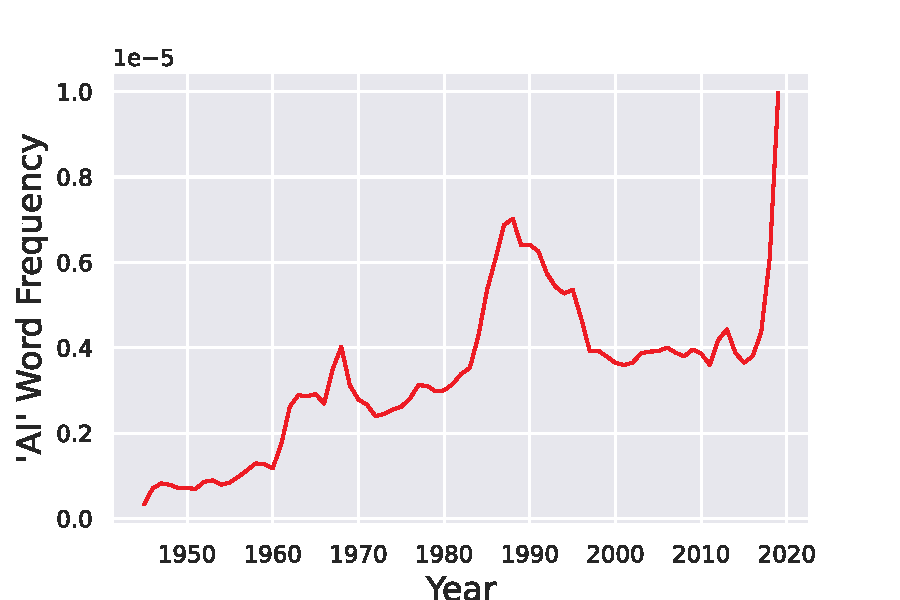
\includegraphics[width=0.7\textwidth]{images/introduction/ngramAI_good.pdf}
    \caption{Γραφική παράσταση της συχνότητας του όρου AI σε βιβλία γραμμένα στην αγγλική γλώσσα ανά έτος (από 1945 μέχρι και 2019). Είναι εμφανείς οι τρεις περίοδοι ακμής του κλάδου. \textit{Παράχθηκε από το \href{https://books.google.com/ngrams}{\en{Google Ngram Viewer}.}} }
\end{figure}



\section{Κίνητρο}
\en{\blindtext[3]}
\section{Συνεισφορά Εργασίας}
\en{\blindtext[3]}
\section{Οργάνωση του Τόμου}

\en{\blindtext[3]} 

    \chapter{Θεωρητικό Υπόβαθρο}

Στο παρόν κεφάλαιο θα οικοδομήσουμε την απαραίτητη γνώση στην οποία βασίζεται η έρευνα των επόμενων ενοτήτων. Αρχικά, θα παρουσιαστούν συνοπτικά τα τεχνητά νευρωνικά δίκτυα \footnote{Από εδώ και στο εξής, με τον όρο \textquote{νευρωνικά δίκτυα} θα αναφερόμαστε στα \textquote{τεχνητά νευρωνικά δίκτυα}.} υπό μια μαθηματική σκοπιά. Έπειτα, θα αναλυθούν τα \hyperlink{_capsule_networks}{νευρωνικά δίκτυα με κάψουλες} (\hyperlink{_capsule_networks}{\en{capsule networks}}) τα οποία και αποτελούν το κύριο θέμα της εργασίας. Τέλος, θα γίνει αναφορά σε νέες τεχνικές και αλγορίθμους που χρησιμοποιήθηκαν στο παρόν έργο ώστε η μετέπειτα εισαγωγή των μεθόδων μας για την εξέλιξη των νευρωνικών δικτύων με κάψουλες να είναι περισσότερο ομαλή και κατανοητή.

\section{Τεχνητά Νευρωνικά Δίκτυα}
Τα σημερινά τεχνητά νευρωνικά δίκτυα, όπως είναι αναμενόμενο, απέχουν σημαντικά από το πρώτο μοντέλο των \en{Warren McCulloch} και \en{Walter Pitts} \cite{mcculloch1943logical} που συζητήσαμε στην ενότητα \ref{sec:historic_note}. Με την ωρίμανση της τεχνολογίας, αυτή ανεξαρτητοποιήθηκε από την \hyperlink{_computational_neuroscience}{(υπολογιστική) νευροεπιστήμη} και εντάχθηκε στην Τεχνητή Νοημοσύνη υπό μια ιεραρχική δομή. Κρίνεται λοιπόν σκόπιμο να παρουσιάσουμε αυτήν την ιεραρχική δομή οργάνωσης της Τεχνητής Νοημοσύνης και μετέπειτα να αναφερθούμε στα επιμέρους στοιχεία της.
\par

\begin{figure}[h]
    \centering
    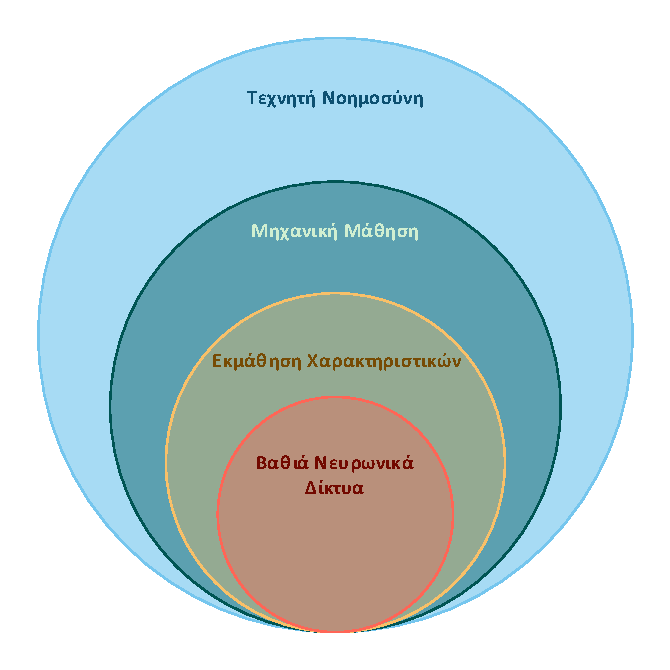
\includegraphics[width=0.7\textwidth]{images/chapter theoritical background/venn ai diagram thesis in greek new 2.pdf}
    \caption{Διάγραμμα \en{Venn} όπου απεικονίζει τη θέση των νευρωνικών δικτύων στην οργάνωση της τεχνητής νοημοσύνης. \textit{Παράχθηκε από το \href{https://www.microsoft.com/en-gb/microsoft-365/visio/flowchart-software/}{\en{Microsoft Visio\texttrademark}.}} }
    \label{fig:_venn_ai}
\end{figure}

Όπως βλέπουμε στο σχήμα \ref{fig:_venn_ai} τα νευρωνικά δίκτυα πολλών επιπέδων (βαθιά νευρωνικά δίκτυα) είναι ένα μέρος του κλάδου της εκμάθησης χαρακτηριστικών (\en{feature learning} ή \en{representation learning}) που είναι ένα μέρος της μηχανικής μάθησης η οποία με τη σειρά της ανήκει στο ευρύτερο επιστημονικό πεδίο της τεχνητής νοημοσύνης. Φυσικά, η τεχνητή νοημοσύνη περιλαμβάνει αρκετούς άλλους κλάδους εκτός από αυτόν της μηχανικής μάθησης\footnote{Βέβαια, ο κλάδος της μηχανικής μάθησης είναι σήμερα ο γρηγορότερα αναπτυσσόμενος.}. Μια χρήσιμη παρατήρηση είναι ότι οι σχέσεις υποσυνόλου συμπίπτουν με τη χρονική αλληλουχία ανάπτυξης του κάθε κλάδου. Δηλαδή, κάθε υποσύνολο αναπτύχθηκε ταυτόχρονα ή αργότερα από το οποιοδήποτε υπερσύνολό του.
\par
Στη συνέχεια, θα γίνει λόγος για τα στοιχεία εκείνα που περιλαμβάνουν την τεχνολογία των βαθιών νευρωνικών δικτύων προκειμένου ο αναγνώστης να αποκτήσει μια εποπτικότερη εικόνα.

\subsection{Μηχανική Μάθηση}


Όπως προδίδει ο όρος, σε αδρές γραμμές τα συστήματα μηχανικής μάθησης έχουν τη δυνατότητα να μαθαίνουν μια εργασία χωρίς να έχουν προγραμματιστεί με ρητές εντολές για τη συγκεκριμένη εργασία αυτή\footnote{Η δυνατότητα αυτή είναι πολύ σημαντική αφού, όπως διαπιστώσαμε στην ενότητα \ref{sec:historic_note} όταν έγινε λόγος για τα έμπειρα συστήματα, για πολλές εργασίες είναι πρακτικός αδύνατο να περιγραφούν ρητά και ντετερμινιστικά οι λύσεις τους.}. Ίσως, ο πιο πλήρης ορισμός δίνεται από τον \en{Tom M. Mitchell} \cite{mitchell1997machine} σύμφωνα με τον οποίο, ένα υπολογιστικό πρόγραμμα λέγεται ότι μαθαίνει από μια εμπειρία \en{E}, ως προς ένα σύνολο εργασιών \en{T} και ένα μέτρο απόδοσης \en{P}, εάν η απόδοσή του σε εργασίες του \en{T}, όπως αυτή μετριέται από το \en{P}, βελτιώνεται με την \en{E}. \footnote{Ο ορισμός αυτός εξηγεί γιατί για παράδειγμα η λήψη μιας ιστοσελίδας της βικιπέδιας και η αποθήκευσή της τοπικά στον υπολογιστή δεν αποτελεί μηχανική μάθηση. Όπως προκύπτει, η \textquote{γνώση} αυτή δεν καθιστά καλύτερο τον υπολογιστή σε κάποια εργασία\cite{geron2019hands}.}
\par

Σύμφωνα με τον ανωτέρω ορισμό διακρίνουμε τρία βασικά συστατικά ενός συστήματος μηχανικής μάθησης. Αυτά είναι τα παρακάτω:
\begin{description}
\item [Εργασία - \en{T}] Είναι το πρόβλημα το οποίο επιθυμούμε να λύσουμε.
\item [Μέτρο Απόδοσης - \en{P}] Αποτελεί μια μετρική του στόχου ως ένδειξη ποιότητας της λύσης μας. Από μαθηματική σκοπιά, είναι αυτό που ο αλγόριθμος μάθησης βελτιστοποιεί.
\item [Εμπειρία - \en{E}] Πρόκειται για τα δεδομένα εισόδου που λαμβάνει το σύστημα υπό τη μορφή παραδειγμάτων ή ως ερεθίσματα ανάδρασης από το περιβάλλον. Όπως θα δούμε στη συνέχεια, ο τρόπος απόκτησης αυτών των δεδομένων αλλά και η φύση τους καθορίζει το είδος της μάθησης.
\end{description}

\subsubsection{Βασικά Είδη Συστημάτων Μηχανικής Μάθησης}
Τα είδη των συστημάτων μηχανικής μάθησης μπορούν να ταξινομηθούν ανάλογα με το:
\begin{itemize}
    \item \emph{Αν εκπαιδεύονται με ανθρώπινη επίβλεψη.}\\
    Ανάλογα με αυτό το κριτήριο έχουμε τις εξής βασικές κατηγορίες: επιβλεπόμενη (\en{supervised}), μη-επιβλεπόμενη (\en{un-supervised}) και ενισχυτική μάθηση (\en{reinforcement learning}).
    \item \emph{Αν μαθαίνουν σταδιακά (\en{incrementally}) και \textquote{στον αέρα} (\en{on the fly}).}\\
    Σε αυτήν την περίπτωση χωρίζουμε τα συστήματα μηχανικής μάθησης σε αυτά που πραγματοποιούν μάθηση σε ζωντανό χρόνο (\en{online learning}) και σε αυτά που μαθαίνουν κατά δέσμες (\en{batch learning}).
    \item \emph{Αν κατασκευάζουν μοντέλα προσαρμοσμένα στα δεδομένα.}\\ 
    Με αυτό το κριτήριο χωρίζονται σε συστήματα βασισμένα σε μοντέλο (\en{model-based}) ή σε συστήματα βασισμένα σε παραδείγματα (\en{instance-based}). \cite{geron2019hands}
\end{itemize}

Προφανώς, κάθε δυνατός συνδυασμός των παραπάνω κριτηρίων είναι αποδεκτός, οδηγώντας έτσι στην ταξινόμηση των συστημάτων μηχανικής μάθησης σε μια πληθώρα από διαφορετικές κατηγορίες. Κρίνεται χρήσιμο, να αναφέρουμε σε όλη την έκταση του έργου τις κατηγορίες στις οποίες ανήκει το κάθε σύστημα που παρουσιάζουμε. Για αυτόν τον λόγο, παροτρύνουμε τον αναγνώστη που δεν είναι εξοικειωμένος με τους ανωτέρω όρους να διαβάσει τους αντίστοιχους ορισμούς στο παράρτημα \ref{chap:definitions}. 
\subsection{Εκμάθηση Χαρακτηριστικών}
Η ανάπτυξη των πρώτων συστημάτων μηχανικής μάθησης απεμπόλησε την ανάγκη των ευφυών εφαρμογών για σχολαστική και ρητή (\en{hard-coded}) αναπαράσταση του χώρου του προβλήματος (π.χ. με την χρήση προτασιακής λογικής). Με τα νέα συστήματα, η γνώση για το πρόβλημα μαθαίνονταν αυτοματοποιημένα μέσω αλγορίθμων μάθησης από το σύνολο δεδομένων εκπαίδευσης. Με άλλα λόγια, τα αλγοριθμικά κατασκευάσματα μάθαιναν να αντιστοιχίζουν με αυτοματοποιημένο τρόπο τα δεδομένα εισόδου (κωδικοποιημένα σε μια μορφή αναπαράστασης) σε τιμές εξόδου. \par

Παρόλα αυτά, τα πρώτα, απλά συστήματα μηχανικής μάθηση δεν έλυσαν όλα τα προβλήματα. Όπως είναι εμφανές από την ανωτέρω περιγραφή, αν και δεν απαιτούνταν η λεπτομερή συγγραφή βάσεων γνώσης, παρέμενε η ανάγκη για αναπαράσταση των δεδομένων εισόδου με μια αποδοτική μορφή. Είναι γεγονός, άλλωστε, ότι η αναπαράσταση σε πολλά συστήματα επηρεάζει καθοριστικά την απόδοση του συστήματος\footnote{Η σημασία της αναπαράστασης δεδομένων στην απόδοση των αλγοριθμικών κατασκευασμάτων δε θα πρέπει να μας εκπλήσσει αφού κάτι αντίστοιχο ισχύει και στους ανθρώπους. Για παράδειγμα, οι περισσότεροι είναι πολύ πιο αποδοτικοί στην αριθμητική χρησιμοποιώντας την αραβική αναπαράσταση αριθμών απ ότι τη λατινική \cite{goodfellow2016deep}.}. Για αυτόν τον λόγο, εξελίχθηκαν διαδικασίες \textquote{μηχανικής χαρακτηριστικών} (\en{feature engineering}) όπου αξιοποιώντας την τεχνική γνώση του χώρου του προβλήματος (\en{domain knowledge}) στόχος είναι η αναπαράσταση των ακατέργαστων δεδομένων εκπαίδευσης ως σύνολο (συνήθως διάνυσμα) από κατάλληλα χαρακτηριστικά. Η καταλληλότητα έγκειται στο πόσο χρήσιμη πληροφορία παρέχουν τα χαρακτηριστικά υπό τον περιορισμό να είναι όσο το δυνατόν περισσότερο ανεξάρτητα μεταξύ τους ώστε να αποπλέκουν (\en{disentagle}) τους παράγοντες διακύμανσης (\en{factors of variation}) των δεδομένων που επηρεάζουν την τιμή εξόδου\cite{goodfellow2016deep}. \par

Οι ανωτέρω έννοιες μπορούν να καταστούν περισσότερο κατανοητές με ένα παράδειγμα συστήματος εκτίμησης τιμών κατοικιών\cite{geron2019hands} (πρόβλημα παλινδρόμησης, επίλυση με επιβλεπόμενη μάθηση κατά δέσμες). Πιο συγκεκριμένα, δοθέντος ενός συνόλου ακατέργαστων δεδομένων που αφορούν την αγορά σπιτιών σε μια περιοχή, το σύστημα, μέσω μηχανικής μάθησης, θα είναι ικανό να εκτιμήσει την τιμή με την οποία μια κατοικία θα πρέπει να κοστολογηθεί για να βγει στην αγορά. ;;Όπως εξηγήσαμε, προτού τροφοδοτήσουμε το σύστημα με το σύνολο δεδομένων, είναι σκόπιμο να εφαρμόσουμε διαδικασίες μηχανικής χαρακτηριστικών σε αυτά και να δημιουργήσουμε μια νέα αναπαράσταση. Τα ακατέργαστα δεδομένα εκπαίδευσης αποτελούνται από μια λίστα όπου κάθε γραμμή αντιστοιχεί σε μια οικία με όλες τις προδιαγραφές της και την τιμή πώλησής της. Στο πρόβλημα του παραδείγματος:
\begin{itemize}
    \item  Ένας παράγοντας διακύμανσης θα μπορούσε να είναι η ακρίβεια της συγκεκριμένης περιοχής. Εντούτοις, σαν προδιαγραφές ας υποθέσουμε ότι αναφέρονται μόνο το γεωγραφικό πλάτος και γεωγραφικό μήκος με αποτέλεσμα η ακρίβεια της περιοχής να μην είναι άμεσα παρατηρήσιμη (συνηθισμένο φαινόμενο στους παράγοντες διακύμανσης). Θα μπορούσαμε λοιπόν να μετατρέψουμε τις συντεταγμένες σε ένα νέο χαρακτηριστικό: την \textquote{κλάση} της περιοχής. Ένας ακόμα παράγοντας διακύμανσης που είναι όμως άμεσα παρατηρήσιμος είναι το εμβαδόν επιφάνειας της κατοικίας.
 \item Μη χρήσιμη πληροφορία θα μπορούσε να είναι ο προσανατολισμός της οικίας. Σε αυτή την περίπτωσή, η δημιουργία μιας νέας αναπαράσταση δεδομένων χωρίς το παρόν προσδιορισμό θα βοηθούσε την επίδοση του συστήματος. 
 \item Δύο αλληλοεξαρτώμενα χαρακτηριστικά (με υψηλή συν\textemdash διακύμανση) θα μπορούσαν να είναι ο αριθμός των υπνοδωματίων και ο αριθμός των μπάνιων όπου τότε η επιλογή της συγχώνευσής τους πιθανότατα βελτίωνε την απόδοση. 
\end{itemize}
\par

Αν και στο παραπάνω πρόβλημα ήταν σχετικά εύκολη η \textquote{χειρονακτική} εξαγωγή χαρακτηριστικών, υπάρχουν πολλοί χώροι προβλημάτων όπου κάτι τέτοιο είναι από πολύ απαιτητικό έως απίθανο. Ενδεικτικά, σε ένα πρόβλημα οπτικής αναγνώρισης ζώων και αντικειμένων (όπως αυτό του \en{CIFAR-10}\cite{cifar10}) είναι εξαιρετικά δύσκολη η περιγραφή χαρακτηριστικών που θα λαμβάνουν μια αναπαράσταση σε εικονοστοιχεία (\en{pixel}) και θα παράγουν μια χρήσιμη αναπαράσταση. \par

Η λύση για την αντιμετώπιση των προβλημάτων της χειρονακτικής εξαγωγής χαρακτηριστικών είναι η χρήση των αλγορίθμων μηχανικής μάθησης για την εκμάθηση όχι μόνο για της αντιστοίχησης των δεδομένων εκπαίδευσης στην επιθυμητή έξοδο αλλά και των ίδιων των αναπαραστάσεων των δεδομένων. Αν και συνήθως, οι προκύπτουσες αναπαραστάσεις μετά τον μετασχηματισμό των ακατέργαστων δεδομένων δεν είναι κατανοητές από τον άνθρωπο, εφόσον η εκπαίδευση γίνει επιτυχημένα, αποτελούνται από χρήσιμα χαρακτηριστικά (που κωδικοποιούν τους παράγοντες διακύμανσης).
Χαρακτηριστικό παράδειγμα συστήματος για την εκμάθηση χαρακτηριστικών είναι ο Αυτοκωδικοποιητής (\en{Autoencoder}).

\subsection{Πολυεπίπεδα Νευρωνικά Δίκτυα}

Η εκμάθηση χαρακτηριστικών σε συνδυασμό με τις ιδέες του κονεκτιβισμού περί κατανεμημένης αναπαράστασης (βλ. ενότητα \ref{sec:historic_note}) μας οδηγεί αναπόφευκτα στη βαθιά μάθηση (\en{deep learning}). Υπό μια αφαιρετική σκοπιά, πρόκειται για τα λεγόμενα \textquote{πολυεπίπεδα νευρωνικά δίκτυα} τα οποία συνδυάζουν τόσο τον μετασχηματισμό της αναπαράστασης των δεδομένων εισόδου όσο και την αντιστοίχηση αυτών των νέων αναπαραστάσεων στην τιμή εξόδου. Τα συστήματα αυτά, όπως θα δούμε στη συνέχεια, είναι δομημένα από απλές υπολογιστικές μονάδες που τους επιτρέπουν να δημιουργούν σύνθετες αναπαραστάσεις μέσω μιας σειράς από εμφωλευμένες, απλούστερες αναπαραστάσεις. Σημειώνουμε ότι πραγματοποιούν μάθηση με κατασκευή μοντέλου (\en{model\textendash based learning systems}) και χρησιμοποιούνται τόσο σε προβλήματα ταξινόμησης όσο και παλινδρόμησης. Στις επόμενες παραγράφους, θα περιγράψουμε με μεγαλύτερη λεπτομέρεια τον χώρο των νευρωνικών δικτύων\footnote{Για έναν τυπικό ορισμό, παραπέμπουμε τον αναγνώστη στο παράρτημα \ref{chap:definitions}}.

\subsubsection{Δομή Απλών Νευρωνικών Δικτύων}
\label{sec:_vanilla_nn}
Τα Νευρωνικά Δίκτυα στην πιο βασική τους μορφή (\en{Feedforward Neural Networks} ή \en{Multilayer Perceptron}) αποτελούνται από απλούς τεχνητούς νευρώνες διασυνδεδεμένους μεταξύ τους με ακμές\textendash βάρη σχηματίζοντας μια πολυεπίπεδη διάταξη. Το πρώτο επίπεδο ονομάζεται επίπεδο εισόδου (\en{input layer}) ενώ το τελευταίο ονομάζεται επίπεδο εξόδου (\en{output layer}). Όλα τα ενδιάμεσα επίπεδα λέγονται κρυφά επίπεδα (\en{hidden layers}) διότι οι τιμές τους δε δίνονται από τα δεδομένα \cite{goodfellow2016deep}. Στην απλή περίπτωση που εξετάζουμε, κάθε κόμβος δέχεται ως είσοδο τιμές από όλους τους κόμβους του αμέσως προηγούμενου επιπέδου (\en{fully connected layer}) και αφού κάνει υπολογισμούς σε αυτές στέλνει το αποτέλεσμα σε όλους τους κόμβους του αμέσως επόμενου επιπέδου.
\par
                  
\begin{figure}[h]
    
    \centering
    \begin{neuralnetwork}[height=4, layerspacing=0.25\textwidth, nodespacing=28mm, nodesize=25pt]
        \newcommand{\mylinktext}[4] {
            % from layer=#1, from node=#2
            % to layer=#3, to node=#4
            $w^{[#3 ]}_{#2#4}$
        }
        % Then assign it:
        \setdefaultlinklabel{\mylinktext}
        \newcommand{\x}[2]{$x_#2$}
        \newcommand{\y}[2]{$\hat{y}_#2$}
        \newcommand{\hfirst}[2]{\small $a^{[1]}_#2$}
        \newcommand{\hsecond}[2]{\small $a^{[2]}_#2$}
        \inputlayer[count=3, bias=false, title=Επίπεδο\\Εισόδου, text=\x]
        \hiddenlayer[count=4, bias=false, title=Κρυφό\\Επίπεδο 1, text=\hfirst] \linklayers
        \hiddenlayer[count=3, bias=false, title=Κρυφό\\Επίπεδο 2, text=\hsecond] \linklayers
        \outputlayer[count=2, title=Επίπεδο\\Εξόδου, text=\y] \linklayers
    \end{neuralnetwork}
    \caption{Διάγραμμα Τεχνητού Νευρωνικού Δικτύου με ένα δύο κρυφά επίπεδα. Οι αγκύλες στους εκθέτες προσδιορίζουν τον αριθμό του επιπέδου. \textit{Παράχθηκε από το \en{LaTeX} πακέτο \href{https://github.com/battlesnake/neural}{\en{neuralnetwork}}. Το πακέτο τροποποιήθηκε και επεκτάθηκε τοπικά.}}
    \label{fig:_vanilla_nn}
\end{figure}

Κοιτώντας κανείς το σχήμα \ref{fig:_vanilla_nn} μπορεί να παρατηρήσει πως οι κόμβοι των επιπέδων εισόδου και εξόδου ξεχωρίζουν από τους κόμβους των κρυφών επιπέδων. Αυτό έχει γίνει για να τονιστεί η ξεχωριστή λειτουργία τους. Πιο συγκεκριμένα, στην περίπτωση του επιπέδου εισόδου, αυτό περιέχει τόσους κόμβους όσος είναι και ο αριθμός των χαρακτηριστικών που περιγράφουν το κάθε παράδειγμα (δηλαδή όσο και το μήκος του διανύσματος εισόδου). Ουσιαστικά, οι κόμβοι εισόδου απλά λαμβάνουν τις τιμές των χαρακτηριστικών και, χωρίς να τις μεταβάλλουν, τις δρομολογούν στους κόμβους του επόμενου επιπέδου. Στην περίπτωση του επιπέδου εξόδου, ο αριθμός των κόμβων είναι τόσος όσος και ο αριθμός των χαρακτηριστικών για την περιγραφή της πρόβλεψης (τόσο όσο το μήκος του διανύσματος εξόδου). Οι κόμβοι εξόδου συνήθως επιβάλουν περιορισμούς στις τιμές των χαρακτηριστικών εξόδου ώστε αυτές να ανήκουν σε ένα φραγμένο σύνολο αριθμών (π.χ. το [0,1]).
\par

Ένα νευρωνικό δίκτυο χωρίς κρυφά επίπεδα δε διαφέρει από έναν γραμμικό ταξινομητή. Είναι γεγονός ότι οι εκπληκτικές δυνατότητες των νευρωνικών δικτύων αποδίδονται στα κρυφά επίπεδα. Χάρη σε αυτά είναι δυνατή η σταδιακή σύνθεση αφηρημένων αναπαραστάσεων από επίπεδο σε επίπεδο που κωδικοποιούν τους παράγοντες διακύμανσης. Τα κρυφά επίπεδα τα απαρτίζουν οι κόμβοι κρυφού επιπέδου\footnote{Εφεξής θα αποκαλούνται ως κόμβοι.}. Ο κάθε ένας από αυτούς υπολογίζει την έξοδο μιας μη γραμμικής συνάρτησης με είσοδο ένα γραμμικό συνδυασμό των τιμών των κόμβων του προηγούμενου επιπέδου. Αξίζει να αναφερθεί στο σημείο αυτό πως δεν υπάρχει κάποιος συγκεκριμένος περιορισμός για τον αριθμό των κόμβων των κρυφών επιπέδων. \par

Η φορμαλιστική περιγραφή των παραμέτρων\footnote{Πρόκειται για μεταβλητές των οποίων οι τιμές μαθαίνονται κατά τη διάρκεια της εκπαίδευσης. Έτσι το νευρωνικό δίκτυο λέμε ότι προσαρμόζεται στα δεδομένα.} και των υπολογισμών που λαμβάνουν χώρα κατά τη διαδικασία πρόβλεψης ενός νευρωνικού δικτύου περιγράφονται παρακάτω. \par

Έστω ένα παράδειγμα εισόδου το οποίο περιγράφεται από \en{\textit{Nx}} χαρακτηριστικά με το διάνυσμα \(X = \big[x_0, x_1, x_2, \dots, x_{Nx}]\). Όλα τα δεδομένα εκπαίδευσης, έστω \en{\textit{M}}, μπορούν να ομαδοποιηθούν σε έναν πίνακα $\boldsymbol{X}$ ως εξής: 
\begin{equation}
    \boldsymbol{X} =
    \underset{(N_x \times M)}{\begin{bmatrix}
        |&|&&| \\
        X^{(1)} & X^{(2)} & \dots & X^{(M)}\\
        |&|&&|
    \end{bmatrix}}.
\end{equation}
\textit{Όπου οι παρενθέσεις στους εκθέτες δηλώνουν τον αριθμό του παραδείγματος.}\par

Αφού προσδιορίσαμε μια μαθηματική αναπαράσταση για τα δεδομένα εισόδου, πάμε να προσδιορίσουμε με φορμαλιστικό τρόπο τις παραμέτρους του νευρωνικού δικτύου. Οι παράμετροι του δικτύου είναι:
\begin{itemize}
    \item Τα βάρη των ακμών (\en{weights}) που συνδέουν δύο διαδοχικά επίπεδα.\\
    \begin{equation}
        \boldsymbol{W} =
        \underset{(N_x \times M)}{\begin{bmatrix}
            |&|&&| \\
            X^{(1)} & X^{(2)} & \dots & X^{(M)}\\
            |&|&&|
        \end{bmatrix}}.
    \end{equation}
    \item Τα δυναμικά πόλωσης (\en{biases}) του κάθε νευρώνα.
\end{itemize}

Τώρα, είμαστε σε θέση να περιγράψουμε τους υπολογισμούς που πραγματοποιεί κάθε νευρώνας\textemdash κόμβος.

\begin{figure}[h]
    \centering
\begin{tikzpicture}[
    init/.style={
      draw,
      circle,
      inner sep=2pt,
      font=\Huge,
      join = by -latex
    },
    squa/.style={
      draw,
      inner sep=2pt,
      font=\Large,
      join = by -latex
    },
    start chain=2,node distance=13mm
    ]
    \node[on chain=2] 
      (x2) {$x_2$};
    \node[on chain=2,join=by o-latex] 
      {$w_2$};
    \node[on chain=2,init] (sigma) 
      {$\displaystyle\Sigma$};
    \node[on chain=2,squa,label=above:{\parbox{2cm}{\centering Activate \\ function}}]   
      {$f$};
    \node[on chain=2,label=above:Output,join=by -latex] 
      {$y$};
    \begin{scope}[start chain=1]
    \node[on chain=1] at (0,1.5cm) 
      (x1) {$x_1$};
    \node[on chain=1,join=by o-latex] 
      (w1) {$w_1$};
    \end{scope}
    \begin{scope}[start chain=3]
    \node[on chain=3] at (0,-1.5cm) 
      (x3) {$x_3$};
    \node[on chain=3,label=below:Weights,join=by o-latex] 
      (w3) {$w_3$};
    \end{scope}
    \node[label=above:\parbox{2cm}{\centering Bias \\ $b$}] at (sigma|-w1) (b) {};
    
    \draw[-latex] (w1) -- (sigma);
    \draw[-latex] (w3) -- (sigma);
    \draw[o-latex] (b) -- (sigma);
    
    \draw[decorate,decoration={brace,mirror}] (x1.north west) -- node[left=10pt] {Inputs} (x3.south west);
    \end{tikzpicture}
    \caption{Διάγραμμα ενός τεχνητού νευρώνα.}
    \label{fig:_neural_node}
\end{figure}
\subsubsection{Συνελικτικά Νευρωνικά Δίκτυα}
\subsubsection{Εκπαίδευση Νευρωνικών Δικτύων}
\subsubsection{Στρατηγικές Βελτίωσης Απόδοσης Νευρωνικών Δικτύων}
\section{Νευρωνικά Δίκτυα με Κάψουλες}
\section{Μηχανισμός Προσοχής}
\section{Μετασχηματιστές}
\section{Χάρτες Αυτο-οργάνωσης}
\label{sec:_SOM}
\section{Αλγόριθμος \en{EM}}
\label{sec:_EM}
\section{Συμπερασματολογία μέσω Διακύμανσης}
% autoencoders

    \blankpage
    % Add Bibliography to contents table.
    \phantomsection 
    \addcontentsline{toc}{chapter}{Βιβλιογραφία}
    % Tell LaTeX where bibliography.bib file is.
    \bibliography{references/bibliography.bib}
    \blankpage
    \appendix
    \chapter{Ορισμοί Εννοιών}
\label{chap:definitions}
Το παρόν παράρτημα περιέχει ορισμούς εννοιών που εισάγονται κατά τη διάρκεια της παρούσας εργασίας. Κατά αυτόν τον τρόπο, δε διακόπτεται η ροή του κυρίως κειμένου. \cite{russell2020artificial,goodfellow2016deep,geron2019hands, bishop2006pattern} 

\begin{description}
    \item[Τεχνητή Νοημοσύνη] \hfill \\ 
    Έχουν υπάρξει πολλοί διαφορετικοί ορισμοί της Τεχνητής Νοημοσύνης: Μερικοί την περιγράφουν σαν εσωτερική διαδικασία της σκέψης που προσομοιάζει αυτής του ανθρώπου ενώ άλλοι ως εξωτερική διαδικασία μαθηματικά βέλτιστης συμπεριφοράς. Σύμφωνα με το κυρίαρχο μοντέλο, η Τεχνητή Νοημοσύνη ασχολείται κυρίως με τη λογική δράση. Ένας ιδανικός ευφυής πράκτορας δρα βέλτιστα σε κάθε περίσταση. Έτσι λοιπόν, η μελέτη της δημιουργίας ευφυών πρακτόρων μπορεί να τεθεί ως ορισμός της Τεχνητής Νοημοσύνης.
    \item[Μηχανική Μάθηση] \hfill \\ 
    Με λίγα λόγια, πρόκειται για τον κλάδο της τεχνητής νοημοσύνης ο οποίος ασχολείται με την ανάπτυξη υπολογιστικών συστημάτων ικανών να μαθαίνουν από παραδείγματα. Αναλυτικότερα, μπορούν και προσαρμόζονται χωρίς να ακολουθούν ρητές εντολές αλλά μέσω αλγορίθμων και στατιστικών μοντέλων που τους επιτρέπουν να αναλύουν και να εξάγουν συμπεράσματα από μοτίβα σε δεδομένα. Χαρακτηριστικό γνώρισμα των συστημάτων μηχανικής μάθησης είναι η ικανότητά τους να βελτιώνουν την απόδοσή τους σε μια εργασία (όπως αυτή μετράται με κάποια κατάλληλη μετρική) όσο η \textquote{εμπειρία} τους σε αυτήν αυξάνεται \cite{mitchell1997machine}.
    \item[Τεχνητά Νευρωνικά Δίκτυα] \hfill \\ 
    Τα τεχνητά νευρωνικά δίκτυα αποτελούν ένα αλγοριθμικό κατασκεύασμα από απλούς υπολογιστικούς κόμβους διασυνδεδεμένους μεταξύ τους μέσω ακμών κάτω από μια συγκεκριμένη τοπολογία (συνήθως οργανώνονται σε επίπεδα, βλ. \ref{sec:_vanilla_nn}). Εμπνευσμένα από τα βιολογικά νευρωνικά δίκτυα, οι κόμβοι μπορούν να παρομοιαστούν με κύτταρα νευρώνων ενώ οι ακμές με νευρικές συνάψεις. \\
    Τα τεχνητά νευρωνικά δίκτυα είναι παράδειγμα συστήματος μηχανικής μάθησης αφού μετά την κατάλληλη εκπαίδευσή τους, γενικεύουν από τα δεδομένα (\en{inference}). Τελικά, μετά την ανάπτυξή τους, υπό μια αφαιρετική σκοπιά αποτελεί το καθένα μια συνάρτηση που αντιστοιχίζει δεδομένα από τον χώρο εισόδου σε \textquote{προβλέψεις} του χώρου εξόδου.
    \item[Βαθιά Μάθηση] \hfill \\ Αποτελεί μια υποκατηγορία μηχανικής μάθησης όπου χρησιμοποιούνται πολυεπίπεδα νευρωνικά δίκτυα. Τα πολλαπλά επίπεδα που διαθέτουν τους επιτρέπουν να μαθαίνουν και να αναγνωρίζουν εσωτερικά, γενικευμένα χαρακτηριστικά των δεδομένων εισόδου.
    \hypertarget{_computational_neuroscience}{
    \item[Υπολογιστική Νευροεπιστήμη (\en{Computational Neuroscience})]} \hfill \\Πρόκειται για τον κλάδο της Νευρωεπιστήμης που χρησιμοποιεί μαθηματικά μοντέλα, μαθηματική ανάλυση και προσεγγιστικά προς τον εγκέφαλο συστήματα για να κατανοήσει τις αρχές ανάπτυξης, δομής, φυσιολογίας καθώς και των γνωστικών (\en{cognitive}) ικανοτήτων του νευρικού συστήματος.
    \item[Επιβλεπόμενη Μάθηση] \hfill \\ Στους αλγορίθμους επιβλεπόμενης μάθησης, ως είσοδος παρέχεται ένα σύνολο δεδομένων μαζί με τους επιθυμητούς στόχους. Δηλαδή, τα δεδομένα δίνονται σε ζεύγη (παράδειγμα εισόδου\textemdash επιθυμητή τιμή εξόδου). Με βάση αυτά, το σύστημα καλείται να εξάγει μια συνάρτηση η οποία θα έχει μάθει να μοντελοποιεί τη σχέση εισόδου\textendash εξόδου μέσα από τα παραδείγματα και τελικά θα είναι ικανή να προβλέψει την τιμή εξόδου σε νέα παραδείγματα για τα οποία η τιμή στόχος είναι άγνωστη. Συνήθως, εκτός από τα δεδομένα για την εκπαίδευση υπάρχουν και άλλα σύνολα δεδομένων για τον έλεγχο της απόδοσης του συστήματος πρόβλεψης.\\
    Ανάλογα με το αν η τιμή στόχος είναι διακριτή ή συνεχής, έχουμε αντίστοιχα το πρόβλημα ταξινόμησης (\en{classification}) ή της παλινδρόμησης (\en{regression}). Παράδειγμα συστήματος ταξινόμησης επιβλεπόμενης μάθησης είναι το φίλτρο ανεπιθύμητης αλληλογραφίας το οποίο αφού εκπαιδεύτηκε με ένα σύνολο επισημασμένων αλληλογραφιών ως ανεπιθύμητων ή επιθυμητών έμαθε να εντοπίζει νέα εισερχόμενη ανεπιθύμητη αλληλογραφία. Ένα παράδειγμα συστήματος παλινδρόμησης επιβλεπόμενης μάθησης είναι αυτό της πρόβλεψης τιμών μετοχών καθώς ο στόχος (κόστος μετοχής) είναι συνεχής αριθμός.

    \item[Μη-επιβλεπόμενη Μάθηση] \hfill \\ Οι αλγόριθμοι μη\textendash επιβλεπόμενης μάθησης, σε αντιδιαστολή με τους αλγορίθμους επιβλεπόμενης μάθησης, δέχονται ως είσοδο ένα σύνολο δεδομένων που περιλαμβάνει παραδείγματα, χωρίς όμως να συνοδεύονται από αντίστοιχες τιμές\textendash στόχους. Στην περίπτωση αυτή, το υπό εκπαίδευση σύστημα επιχειρεί να μάθει πρότυπα στα δεδομένα εισόδου χωρίς κάποιο μηχανισμό ανατροφοδότησης. Συνήθεις εφαρμογές μη\textendash επιβλεπόμενης μάθησης είναι αυτές της ομαδοποίησης των δεδομένων σε συστάδες ή της αναπαράστασής τους με ένα γράφημα.
    
    \item[Ενισχυτική Μάθηση] \hfill \\ Στην ενισχυτική μάθηση, στο σύστημα (το οποίο καλείται \textquote{ευφυής πράκτορας} στο πλαίσιο αυτό) δεν παρέχεται κάποιο σύνολο δεδομένων αλλά η όποια εμπειρία αποκτάται μέσω της αλληλεπίδρασής του με το περιβάλλον. Ο πράκτορας έχει τη δυνατότητα να παρατηρήσει το περιβάλλον του και τη (πιθανή) κατάστασή του και ανάλογα με μια στρατηγική (\en{policy}) να δράσει σε αυτό. Το περιβάλλον του, με κάθε δράση (και ανάλογα την κατάσταση) παρέχει την απαραίτητη εμπειρία υπό τη μορφή επιβράβευσης (\en{reward}) ή ποινής (\en{punishment}). Έτσι, ο πράκτορας μαθαίνει από την εμπειρία προσαρμόζοντας τη στρατηγική του ώστε να μεγιστοποιεί την επιβράβευση την οποία λαμβάνει και τελικά να πετυχαίνει τον στόχο του. Παράδειγμα ενός τέτοιου πράκτορα είναι ένα σύστημα το οποίο παίζει σκάκι.

    \item[Μάθηση Κατά Δέσμες] \hfill \\ Αφορά το είδος συστημάτων μηχανικής μάθησης που δεν έχουν τη δυνατότητα να μαθαίνουν σταδιακά αλλά εκπαιδεύονται μονομιάς χρησιμοποιώντας όλο το σύνολο δεδομένων στην είσοδό τους. Σε περίπτωση που προστεθούν νέα δεδομένα στα οποία θα επιθυμούσαμε το σύστημα να προσαρμοστεί, απαιτείται εκ νέου εκπαίδευση στο καινούριο σύνολο δεδομένων το οποίο θα περιέχει τόσο τα παλαιά όσο και τα επιπρόσθετα δεδομένα (διαδικασία χρονοβόρα και υπολογιστικά κοστοβόρα). Συνήθως, σε τέτοιες περιπτώσεις το σύστημα πρέπει να σταματήσει να λειτουργεί και να μεταβεί στη φάση σχεδιασμού. Παραδείγματα αυτών των μεθόδων αποτελούν ο αλγόριθμος \en{Expectation Maximization} και ο \en{Self-organizing map} όπως περιγράφεται στην ενότητα \ref{sec:_SOM}.
    
    \item[Μάθηση σε Ζωντανό Χρόνο] \hfill \\ Πρόκειται για τα συστήματα μηχανικής μάθησης που, σε αντίθεση με αυτά που μαθαίνουν κατά δέσμες, είναι ικανά να εκπαιδεύονται σταδιακά, είτε με ένα παράδειγμα τη φορά είτε με μικρές δέσμες παραδειγμάτων στην είσοδό τους. Το θετικό σε αυτά τα συστήματα είναι η δυνατότητα προσαρμογής τους σε νέα δεδομένα με πολύ μικρό χρονικό και υπολογιστικό κόστος. Αποτέλεσμα αυτού είναι ότι υπάρχει (συνήθως) η δυνατότητα η εκπαίδευσή τους να γίνει ζωντανά (\en{online}) χωρίς να σταματήσει η λειτουργία του συστήματος. Παράδειγμα αποτελούν οι εφαρμογές πρόβλεψης τιμών μετοχών όπου απαιτείται συνεχής προσαρμογή του συστήματος στα νέα δεδομένα της αγοράς. 
    
    \item[Μάθηση Βασισμένη σε Παραδείγματα] \hfill \\ Είναι μια οικογένεια απλών συστημάτων μηχανικής μάθησης που αφορά τον τρόπο με τον οποίο ένα σύστημα γενικεύει από τα παραδείγματα του συνόλου εισόδου. Στα συγκεκριμένα, όταν τα τροφοδοτούμε με κάποιο νέο παράδειγμα, το συγκρίνουν με τα δεδομένα εισόδου (ή ένα υποσύνολο αυτών) τα οποία έχουν αποθηκευθεί στη μνήμη τους κατά την εκπαίδευση. Ένα χαρακτηριστικό μειονέκτημα αυτών των συστημάτων είναι ότι ο χώρος που απαιτείται για την αποθήκευση του μοντέλου (του συστήματος μάθησης μετά την εκπαίδευσή του) αυξάνεται με το μέγεθος του συνόλου εισόδου (συνήθως με γραμμικό τρόπο). Ενδεικτικά, ένα σύστημα που γενικεύει κατά αυτόν τον τρόπο είναι το \en{K-nearest neighbors}.
    
    \item[Μάθηση Βασισμένη σε μοντέλο] \hfill \\ Είναι μια άλλη οικογένεια συστημάτων όπου η μηχανική μάθηση γίνεται μέσω της προσαρμογής (\en{fitting}) ενός μοντέλου στα δεδομένα εισόδου. Έχοντας εκφράσει το σύνολο των δεδομένων εκπαίδευσης (ή τη σχέση αυτών με την επιθυμητή έξοδο) χρησιμοποιώντας ένα κατάλληλα εκφραστικό (\en{expressive}) μοντέλο, λέμε ότι το σύστημα μαθαίνει να \textquote{γενικεύει} από τα παραδείγματα. Έτσι, για να παράξει προβλέψεις σε νέα δεδομένα, δεν απαιτείται η αποθήκευση όλων των δεδομένων εκπαίδευσης αλλά μόνο των παράμετρων του μοντέλου που εκφράζει.

    \item[Γνωστική Νευρoεπιστήμη] \hfill \\ Η Γνωστική νευρωεπιστήμη είναι το πεδίο μελέτης που ασχολείται με τα νευρωνικά υποστρώματα των διανοητικών διεργασιών. Είναι η τομή της ψυχολογίας με τη νευροεπιστήμη. Συνδυάζει τις θεωρίες της γνωστικής ψυχολογίας και της υπολογιστικής μοντελοποίησης με πειραματικά δεδομένα του εγκεφάλου.
    
    \item[Αναγνώριση Προτύπων] \hfill \\ Είναι ένα επιστημονικό πεδίο με στόχο την ανάπτυξη αλγορίθμων για την αυτοματοποιημένη απόδοση κάποιας τιμής (παλινδρόμησης) ή διακριτικού στοιχείου (ταξινόμηση) με βάση μοτίβα/χαρακτηριστικά που παρατηρούνται στα εισαγόμενα δεδομένα, συνήθως κωδικοποιημένα ως αλληλουχίες αριθμών.  
    \item[Γραμμικά Διαχωρίσιμες Κλάσεις] \hfill \\ Λέμε ότι ένα σύνολο δεδομένων για ταξινόμηση που περιέχει δύο κλάσεις είναι γραμμικά διαχωρίσιμο αν και μόνο αν μπορούμε να διαχωρίσουμε τις δύο κλάσεις στον πολυδιάστατο χώρο χαρακτηριστικών εισόδου χρησιμοποιώντας ένα υπερεπίπεδο. Στην περίπτωση όπου ο χώρος χαρακτηριστικών είναι δισδιάστατος, αρκεί να μπορούμε να χαράξουμε μια ευθεία γραμμή στο καρτεσιανό επίπεδο που να διαχωρίζει τις δύο κλάσεις.
    
    \item[Γραμμικά Μοντέλα] \hfill \\ Τα γραμμικά μοντέλα περιγράφουν τη σχέση μεταξύ ενός ή περισσοτέρων μεταβλητών εισόδου (μεταβλητές πρόβλεψης) και μιας συνεχούς τιμής εξόδου (απόκρισης). Η χρήση των μοντέλων αυτών ενδείκνυται όταν οι σχέσεις μεταξύ εισόδου\textendash εξόδου είναι (σχεδόν) γραμμικές στο διάστημα μελέτης. Μια στατιστική μέθοδος για την παραγωγή γραμμικών μοντέλων που μοντελοποιούν αυτές τις σχέσεις από σύνολα δεδομένων εισόδου\textendash εξόδου είναι η γραμμική παλινδρόμηση.
     
    \item[Γενετικοί Αλγόριθμοι] \hfill \\ Οι Γενετικοί αλγόριθμοι ανήκουν στο κλάδο της επιστήμης υπολογιστών και αποτελούν μια μέθοδο αναζήτησης βέλτιστων λύσεων σε προβλήματα βελτιστοποίησης. Είναι χρήσιμοι σε περιπτώσεις όπου ο χώρος αναζήτησης λύσης είναι πολύ μεγάλος και δεν υπάρχει αναλυτική μέθοδος που να μπορεί να βρει το βέλτιστο συνδυασμό τιμών των μεταβλητών του προβλήματος ώστε το υπό εξέταση σύστημα να αντιδρά με βέλτιστο τρόπο. Ο τρόπος λειτουργίας των Γενετικών Αλγορίθμων είναι εμπνευσμένος από τη βιολογία. Χρησιμοποιεί δηλαδή την ιδέα της εξέλιξης μέσω γενετικής μετάλλαξης, φυσικής επιλογής και διασταύρωσης. Για να αξιοποιήσουμε αυτές τις ιδέες, κωδικοποιούμε κάθε πιθανή λύση του προβλήματος σαν ένα συγκεκριμένο γονιδίωμα και ξεκινάμε από έναν τυχαίο πληθυσμό τέτοιων λύσεων/γονιδιωμάτων. Έπειτα, ορίζοντας μια συνάρτηση ικανότητας (\en{fittness function}) που περιγράφει την ποιότητα της λύσης είμαστε σε θέση να αφήσουμε τον μηχανισμό εξέλιξης να δράσει για ορισμένες γενιές ώστε τελικά να έχουν απομείνει και πολλαπλασιαστεί γονιδιώματα που περιγράφουν (σχεδόν) βέλτιστες λύσεις. Οι γενετικοί αλγόριθμοι δεν εγγυώνται την εύρεση της βέλτιστης λύσης.
    
    \hypertarget{_capsule_networks}{
    \item[Νευρωνικά Δίκτυα με Κάψουλες (\en{Capsule Networks})]} \hfill \\ Πρόκειται για βαθιά νευρωνικά δίκτυα που επιδιώκουν να πραγματοποιήσουν ανάστροφα γραφικά για να λύσουν κυρίως προβλήματα αναγνώρισης αντικειμένων σε εικόνες. Αποτελούνται από επίπεδα από κάψουλες. Κάθε κάψουλα είναι σαν μια συνάρτηση η οποία προσπαθεί να προβλέψει τις παραμέτρους στιγμιοτύπου (π.χ. προσανατολισμός, θέση κ.τ.λ.) ενός συγκεκριμένου αντικειμένου και την πιθανότητα ύπαρξής του σε μια περιοχή της εικόνας (δηλαδή στο πεδίο υποδοχής της κάψουλας).
    
    \item[Γραφικά Υπολογιστή] \hfill \\ Αφορά τον κλάδο της επιστήμης υπολογιστών που μελετά μεθόδους για ψηφιακή σύνθεση και χειρισμό οπτικού περιεχομένου. Εμπεριέχει μια δόση τέχνης αφού σχετίζεται με τον σχεδιασμό του περιεχομένου αυτού.
    
    \item[Απόδοση Εικόνας (\en{Rendering})] Είναι η διεργασία δημιουργίας εικόνας από ένα μοντέλο δύο ή τριών διαστάσεων με τη χρήση ενός προγράμματος υπολογιστή. Πολλά μοντέλα ορίζονται σε ένα αρχείο σκηνής (\en{scene file}) το οποίο περιγράφει όλη την πληροφορία της οπτικής σκηνής που θα παραχθεί με την απόδοση εικόνας. Συνήθως, το αρχείο σκηνής περιέχει πληροφορία για τη γεωμετρία, την οπτική γωνία, την υφή, τον φωτισμό και τη σκίαση των αντικειμένων.
    
    \item[Ανάστροφα Γραφικά] \hfill \\ Πρόκειται για την ανάστροφη διαδικασία της απόδοσης εικόνας. Δηλαδή, δοθείσης μιας οπτικής εικόνας, να προσδιοριστεί το αρχείο σκηνής από το οποίο δημιουργήθηκε.
    
    \item[Ακολουθιακά Δεδομένα (\en{Sequential Data})] \hfill \\ Ο όρος αφορά δεδομένα των οποίων τα επιμέρους στοιχεία διατάσσονται σε μια συγκεκριμένη σειρά. Για παράδειγμα, οι λέξεις στον φυσικό λόγο αποτελούν ακολουθιακά δεδομένα. Άλλα παραδείγματα είναι οι ακολουθίες DNA και η τιμή μιας μετοχής στο χρηματιστήριο, όπως αυτή μεταβλαλλεται στον χρόνο.
    \item[Κανονικοποίηση Επιπέδου (\en{Layer Normalization})] \hfill \\ Πρόκειται για μια τεχνική που χρησιμοποιείται για την κανονικοποίηση της κατανομής των τιμών ενεργοποίησης σε κάθε παράδειγμα εισόδου ξεχωριστά \cite{ba2016layer_normalization}. Η τεχνική αυτή μειώνει σημαντικά τον χρόνο εκπαίδευσης (οι συναρτήσεις ενεργοποίησης λειτουργούν στη γραμμική περιοχή τους, γύρω από το μηδέν).
    \item[Ανταγωνιστική Μάθηση (\en{Competitive Learning})] \hfill \\ Αφορά την διαδικασία μη\textendash επιβλεπόμενης μάθησης κατά την οποία διαφορετικοί νευρώνες (ή γενικότερα, υπολογιστικές μονάδες) ανταγωνίζονται για το ποιός θα αναλάβει να \textquote{εξηγήσει} και να μάθει να αναπαριστά την εκάστοτε είσοδο $x_i$ (ενός συνόλου εδομένων). Από την στιγμή που όλοι οι νευρώνες, καθώς το δίκτυο τροφοδοτείται με παραδείγματα, μαθαίνουν να αναπαριστούν καλύτερα τις εισόδους που είναι ήδη καλοί στο να αναπαριστούν, εξειδικεύονται στο να εξηγούν συγκεκριμένα μοτίβα εισόδων ο καθένας. Μια από τις πιο απλές μορφές της ανταγωνιστικής μάθησης είναι η λεγόμενη \textquote{ο νικητής τα παίρνει όλα} (\en{winner takes it all}), όπως παρουσιάζεται στην ενότητα \ref{sec:_SOM} \cite{sammut2011encyclopedia}.
    \item[Αυτοκωδικοποιητής (\en{Autoencoder})] Πρόκειται για μια αρχιτεκτονική τεχνητών νευρωνικών δικτύων που χρησιμοποιείται για την εκμάθηση αποδοτικών (διανυσματικών) αναπαραστάσεων από μη\textendash σεσημασμένα δεδομένα. Σε αυτό το είδος του νευρωνικού δικτύου, δίνεται σαν είσοδος ένα παράδειγμα (διάνυσμα χαρακτηριστικών) και απαιτούμε να λάβουμε στην έξοδο το ίδιο διάνυσμα (μέσω μιας συνάρτησης σφάλματος η οποία συγκρίνει την έξοδο με την είσοδο). Με λίγα λόγια, εκπαιδεύουμε το δίκτυο ώστε να έχει συμπεριφορά ταυτοτικής συνάρτησης. Ο περιορισμός όμως είναι ότι ανάμεσα στο επίπεδο εισόδου και το επίπεδο εξώδου επιβάλουμε (μέσω αρχιτεκτονικής) μια στένωση (bottleneck) με το να χρησιμοποιούμε λιγότερους κόμβους κρυφών επιπέδων από τους κόμβους εισόδου και εξόδου. Έτσι, το δίκτυο μαθαίνει συμπικνωμένες αναπαραστάσεις των δεδομένων. 
 \end{description}
    \chapter{Απόδοση Ξενόγλωσσων Όρων}
\begin{center}
\begin{tabular}{ll}
    \large{\textbf{\underline{Ξενόγλωσσος όρος}}} & \large{\textbf{\underline{Ελληνική απόδοση}}}\\
    
    \en{batch learning} & μάθηση κατά δέσμες\\
    \en{online learning} & μάθηση σε ζωντανό χρόνο\\
    \en{supervised learning} & επιβλεπόμενη μάθηση\\
    \en{unpervised learning} & μη-επιβλεπόμενη μάθηση\\
    \en{reinforcement learning} & ενισχυτική μάθηση\\
    \en{capsule networks} & νευρωνικά δίκτυα με κάψουλες\\
    \en{instance based} & βασισμένο σε παραδείγματα\\
    \en{perturbation test} & πείραμα διαταραχής\\
    \en{learning rate} & ρυθμός μάθησης\\
    \en{optimizer} & βελτιστοποιητής\\
    \en{multihead attention} & πολυκέφαλη προσοχή\\
    \en{equivariant} & ισομεταβλητό \\
    \en{invariant} & ανεξάρτητο \\
    \en{recurrent neural network} & επαναλαμβανόμενο νευρωνικό δίκτυο\\
    \en{reconstructor} & ανακατασκευαστής\\
    \en{inverse graphics} & ανάστροφα γραφικά\\


\end{tabular}
\end{center}


    \chapter{Συντομογραφίες - Ακρωνύμια}

\section{Ελληνικά}

\begin{flushleft}
    \begin{tabular}{ll}
        \large{\textbf{\underline{Συντομογραφία ή Ακρωνύμιο}}} & \large{\textbf{\underline{Πλήρης όρος}}} \\
        
        dfjfewrgerrewgte & gvsdf ergwegfewrftweg\\
        dfjfewrgergergrewgte & gvsgfewrftweg\\
        dfjfewrgegte & gvsdf ewrftweg\\
        dfjfewrgerregergergtergvgergrewgte & gvsdf ergwegfewrftwegegergergerwgerf
    \end{tabular}
    \end{flushleft}

\section{Αγγλικά}

\begin{flushleft}
    \begin{tabular}{ll}
        \large{\textbf{\underline{Συντομογραφία ή Ακρωνύμιο}}} & \large{\textbf{\underline{Πλήρης όρος}}} \\
        
        dfjfewrgerrewgte & gvsdf ergwegfewrftweg\\
        dfjfewrgergergrewgte & gvsgfewrftweg\\
        dfjfewrgegte & gvsdf ewrftweg\\
        dfjfewrgerregergergtergvgergrewgte & gvsdf ergwegfewrftwegegergergerwgerf
    \end{tabular}
    \end{flushleft}


    
    
\end{document}